\documentclass[11pt,english,french]{scrreprt}
\usepackage{lmodern}
\usepackage{babel}
\renewcommand{\familydefault}{\rmdefault}
\usepackage[T1]{fontenc}
\usepackage{ucs}
\usepackage[utf8x]{inputenc}
\usepackage[a4paper]{geometry}
\geometry{verbose,tmargin=3cm,bmargin=3cm,lmargin=2cm,rmargin=2cm,headheight=2cm,footskip=2cm}
\setlength{\parskip}{\smallskipamount}
\setlength{\parindent}{0pt}

\usepackage[titles]{tocloft}
\usepackage{abstract}
\usepackage{amsthm}
\usepackage{booktabs}
\usepackage{amsmath}
\usepackage{amssymb}
\usepackage[unicode=true, pdfusetitle,
 bookmarks=true,bookmarksnumbered=false,bookmarksopen=false,
 breaklinks=false,pdfborder={0 0 1},backref=false,colorlinks=false]
 {hyperref}

\makeatletter
\usepackage{colortbl}
\usepackage{color}
\usepackage[dvipsnames]{xcolor}
\usepackage{listings}
\usepackage[calcwidth]{titlesec}
\usepackage{fix-cm}
\usepackage{multicol}
\usepackage{wrapfig}
\usepackage{graphicx}
\usepackage{tabularx}
\graphicspath{{images/}}
\usepackage{algorithm,algorithmic}
\usepackage{nicefrac}
\usepackage{verbatim}
\usepackage{moreverb}
\usepackage{subfig}
\usepackage[strict]{changepage}
\usepackage{pdflscape}

\newcounter{cptPb}
\setcounter{cptPb}{1}

\theoremstyle{remark}
  \newtheorem*{rem*}{Remarque}
  \newtheorem*{ex*}{Exemple}
\theoremstyle{definition}
  \newtheorem*{def*}{Définition}
  \newtheorem*{obj*}{Objectif}
  \newtheorem*{idee*}{Idée}
  \newtheorem*{ppe*}{Principe}
  \newtheorem*{ccl*}{Conclusion}
  \newtheorem{pb}{Problème}[cptPb]
  \newtheorem*{pb*}{Problème}
\definecolor{MyDarkBlue}{rgb}{0,0.08,0.45}

\lstset{language=C,
	 	basicstyle=\small\ttfamily,
		keywordstyle=\ttfamily\textcolor{RubineRed},
		identifierstyle=,
		commentstyle=\textcolor{OliveGreen},
		columns=fullflexible,
		stringstyle=\sffamily\textcolor{BurntOrange},
		showstringspaces=false,numberstyle=\tiny, breaklines=true,
		morekeywords={bool,false,true}}

\titleformat{\section}[hang]{\sffamily\bfseries}
 {\Large\thesection}{12pt}{\Large}[{\titlerule[0.5pt]}]

\titleformat{\subsection}[hang]{\sffamily\bfseries}
 {\large\thesubsection}{12pt}{\large}

\def\thickhrulefill{\leavevmode \leaders \hrule height 1pt\hfill \kern \z@}

\makeatletter
\def\maketitle{%
  \null
  \thispagestyle{empty}%
  \vfill
  \begin{center}\leavevmode
    \normalfont
    {\huge \sffamily \bfseries\color{orange}\raggedright \@title\par}%
    \thickhrulefill\par
    {\large\sffamily\color{MyDarkBlue}\raggedleft \@author\par}%
    \vskip 1cm
    {\Large \sffamily \@date\par}%
	{\Large \sffamily \@blurb\par}%
  \end{center}%
  \vfill
  \null
  \cleardoublepage
  }

\def\blurb#1{\def\@blurb{#1}}

\AtBeginDocument{
  \def\labelitemi{\normalfont\bfseries{--}}
}
\renewcommand{\abstractname}{Introduction}
\renewcommand{\abstractnamefont}{\Large\sffamily\bfseries}
\renewcommand{\absnamepos}{flushleft}

\setlength{\cftbeforesecskip}{0.5ex}
\setlength{\cftbeforepartskip}{2ex}
\setlength{\cftsecindent}{1cm}
\renewcommand{\cftsecfont}{\mediumsize \sffamily \bfseries}
\renewcommand{\cftsecdotsep}{\cftdotsep}      

\newcommand*\Pitem{%
  \item[\color{green}\scalebox{0.9}{\textbullet}]}
\newcommand*\Citem{%
  \item[\color{red}\scalebox{0.9}{\textbullet}]}


\setcounter{tocdepth}{1}

\usepackage{remreset}
\makeatletter 
\@addtoreset{section}{part}
\@addtoreset{section}{chapter} 
\makeatother

\def\@part[#1]#2{%
      \ifnum \c@secnumdepth >\m@ne
        \refstepcounter{part}%
        \addcontentsline{toc}{part}{\thepart\hspace{1em}#1}%
      \else
        \addcontentsline{toc}{part}{#1}%
      \fi
      {\parindent \z@ \raggedright
       \interlinepenalty \@M
       \normalfont
       \ifnum \c@secnumdepth >\m@ne
         \Large \sffamily \bfseries \partname~\thepart
         \par\nobreak
       \fi
       \huge \sffamily \bfseries #2%
       \markboth{}{}\par}%
      \nobreak
      \vskip 5ex
      \@afterheading}
  \def\@spart#1{%
      {\parindent \z@ \raggedright
       \interlinepenalty \@M
       \normalfont
       \huge \sffamily \bfseries #1\par}%
       \nobreak
       \vskip 3ex
       \@afterheading}

\makeatother

\makeatletter
\def\@makechapterhead#1{%
  \vspace*{10\p@}%
  {\parindent \z@ \raggedright
    \normalfont
    \ifnum \c@secnumdepth >\m@ne
      \if@mainmatter
        %\huge\bfseries 
        \scshape
        \@chapapp\space \thechapter
        \par\nobreak
%        \vskip 20\p@
      \fi
    \fi
    \interlinepenalty\@M
    \Huge \bfseries \sffamily #1\par\nobreak
    \vskip 40\p@
  }}
\def\@schapter#1{\if@twocolumn
                   \@topnewpage[\@makeschapterhead{#1}]%
                 \else
                   \@makeschapterhead{#1}%
                   \@afterheading
                 \fi}
\def\@makeschapterhead#1{%
  \vspace*{10\p@}%
  {\parindent \z@ \raggedright
    \normalfont
    \scshape
    \interlinepenalty\@M
    \Huge \bfseries \sffamily #1\par\nobreak
    \vskip 40\p@
  }}

\makeatother


\begin{document}
\author{BARON Benjamin}
\date{Le \today}
\blurb{D'après le cours de \href{http://pagesperso-systeme.lip6.fr/Pierre.Sens/}{Pierre Sens}}

\title{LI324 - Notes de cours\\
Introduction aux systèmes d'exploitation}

%\begin{landscape}
\maketitle
%\end{landscape}
\renewcommand\contentsname{\vspace{-30pt}Table des matières\vspace{-30pt}} 
\tableofcontents

\chapter{Introduction} % (fold)

\section{Historique} % (fold)

\paragraph{1940} % (fold)
Ordinateur à tubes. Il n'y a pas de système. 
\begin{ex*}
	ENIAC : \textasciitilde $20\,000$ tubes $\Rightarrow$ 2 octets
\end{ex*}

\paragraph{1960} % (fold)
Ordinateur à transistors composé d'un \emph{mainframe} (gros système).
\begin{ex*}
	ATLAS (60) : traitement par lots (\emph{batch})
\end{ex*}
\begin{figure}[h!]
	\center
	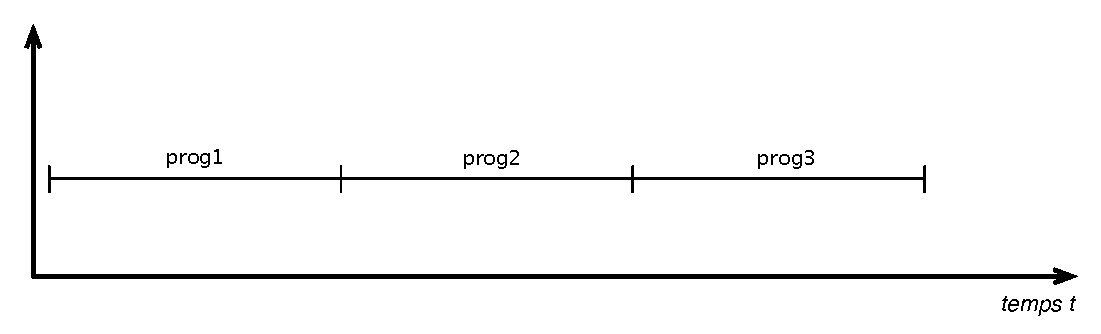
\includegraphics[scale=.6]{img/batch}
\end{figure}

\paragraph{1962} % (fold)
Mainframe à temps partagé (\emph{time sharing}) : CTSS (MIT). Il y a un partage du temps pour tous les programmes : \emph{quantum} alloué pour chaque programme.

\begin{ex*}
	MUTICS (65), OS1360 (IBM, 64)\\
	+100 utilisateurs pour un ordinateur
\end{ex*}

\begin{figure}[h!]
	\center
	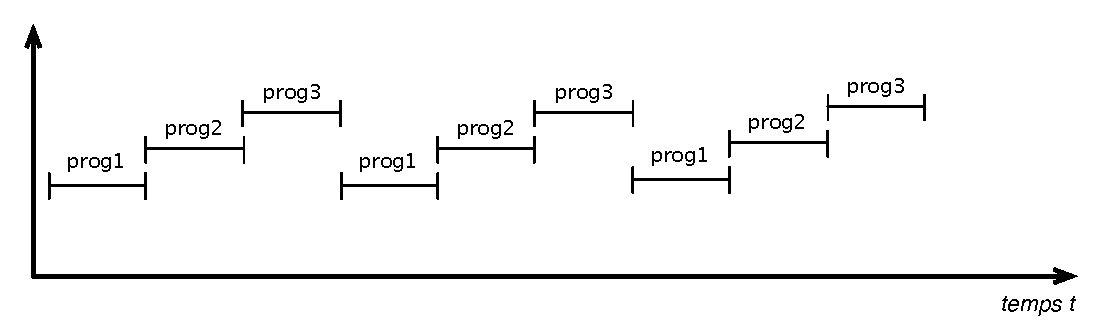
\includegraphics[scale=.6]{img/split-time}
\end{figure}

\paragraph{1969} % (fold)
Mini-ordinateur : UNICS $\rightarrow$ UNIX

+10 utilisateurs pour un ordinateur, temps partagé, systèmes en langage machine (assembleur)

\paragraph{1973} % (fold)
Langage C pour ré-écrire UNIX. Il a fallu environ $10\,000$ lignes de code C pour écrire le premier système d'exploitation UNIX.

\paragraph{1980} % (fold)
Micro-ordinateur (ordinateur dédié à un utilisateur particulier). Il s'agit d'\textbf{une} station de travail pour \textbf{un} utilisateur. 
\begin{ex*}
	Systèmes d'exploitation pour PC (\emph{Personnal Computer}) \textasciitilde batch : CP/M, MS-DOS\dots
\end{ex*}

\paragraph{1990 -- 91} % (fold)
UNIX pour PC (\emph{opensource}) : Mimix, Linx, FreeBSD


\paragraph{1993} % (fold)
MS-DOS devient Windows (équivalent au batch : mono-tâche, mono-utilisateur).

La branche NT de Windows crée Windows NT, un système d'exploitation multi-tâches, multi-utilisateurs

\paragraph{2000} % (fold)
Fin de la branche ``MS-DOS -- Windows'' (3.1, 95, 98, Millenium) de Microsoft. Seule la branche NT de Microsoft subsiste (NT, NT4, 2000).

\paragraph{2009} % (fold)
Sortie de Windows 7 (NT)

NT $\rightarrow$ 2000 $\rightarrow$ XP $\rightarrow$ Vista $\rightarrow$ Windows 7 (NT)

\section{Définitions}

\begin{def*}[Programme]
	Expression d'un algorithme à l'aide d'un langage de programmation.
\end{def*}

\begin{def*}[Tâche]
	Conjonction d'un programme et des données auxquelles il s'applique.
\end{def*}

\begin{def*}[Processus]
	Un processus est l'exécution d'une tâche. Il est caractérisé par la \textbf{tâche} et son \textbf{contexte d'exécution}, c'est-à-dire la valeur du compteur ordinal, les valeurs des registres, etc.
\end{def*}

\begin{def*}[Monoprogrammation vs. multiprogrammation]
	En monoprogrammation, il y a un seul processus à la fois en mémoire. Lorsqu'une tâche est soumise et que le processeur est disponible, on la charge en mémoire puis on exécute le processus associé jusqu'à ce qu'il soit terminé. On passe alors à la tâche suivante.
	
	En multiprogrammation, il peut y avoir plusieurs processus à la fois en mémoire. Une tâche soumise est chargée en mémoire s'il y a de la place et donne naissance à un processus. Un processus est prêt s'il n'est pas en attente d'un événement extérieur (fin d’entrée-sortie, libération de ressource, etc.). \\
	Les processus prêts s'exécutent à tour de rôle, on parle de commutation de processus. 
	\begin{rem*}
		La multiprogrammation peut être utilisée en batch ou en temps partagé.
	\end{rem*}
\end{def*}

\begin{def*}[Batch vs. temps partagé]
	En batch, il n'y a commutation que si le processus actif doit effectuer une entrée-sortie. 
	
	En temps partagé, il y a commutation si le processus actif est en attente d’un événement ou	s'il a épuisé son quantum. Un quantum est une durée élémentaire (de l'ordre de 10 à 100 ms).
\end{def*}

\begin{def*}[\emph{Overhead}]
	Temps passé (perdu) à effectuer une commutation entre deux processus en temps partagé.
\end{def*}

\begin{def*}[Unité d'échange]
	Une unité d'échange sert à effectuer des transferts entre la mémoire principale et un périphérique sans utiliser le processeur (DMA -- \emph{Direct Memory Access}). Elle reçoit un ordre du processeur, effectue le transfert, puis avise le processeur de la fin de l'échange. Durant le transfert, le processeur peut faire d'autres calculs.
\end{def*}

\clearpage

\section{Composants d'un ordinateur} % (fold)
\subsection{Architecture de base} % (fold)

\begin{figure}[h!]
	\center
	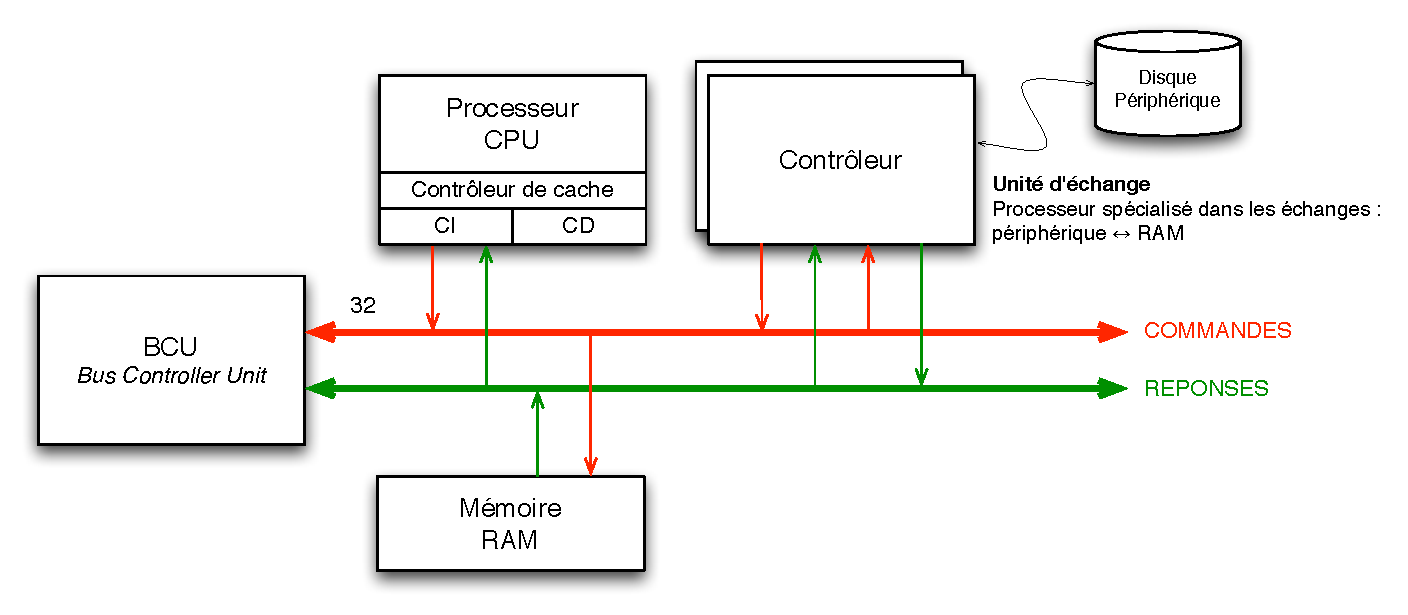
\includegraphics[scale=.6]{img/architecture}
\end{figure}

\begin{rem*}
	Il y a un vrai parallélisme entre les traitements sur le CPU et les traitements sur les contrôleurs (qui sont des processeurs spécialisés).
\end{rem*}

\subsection{Hiérarchie des temps d'accès} % (fold)
\begin{figure}[h!]
	\center
	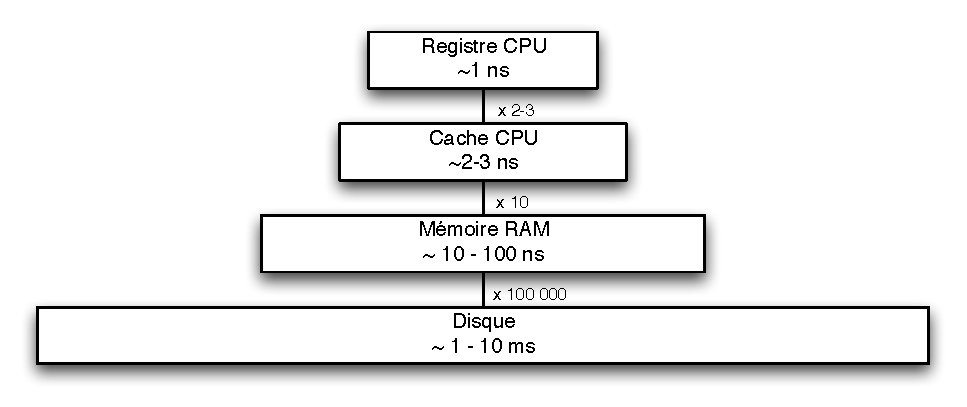
\includegraphics[scale=.75]{img/hierarchie-memoire}
\end{figure}

\clearpage

\section{Les systèmes d'exploitation} % (fold)

Un système d'exploitation (ou OS -- \emph{Operating System}) est :\begin{itemize}
	\item Un programme qui gère l'ordinateur ;
	\item Un programme qui donne la vision d'une machine virtuelle (cache la complexité de la machine).
\end{itemize}

\subsection{Architecture} % (fold)
\begin{figure}[h!]
	\center
	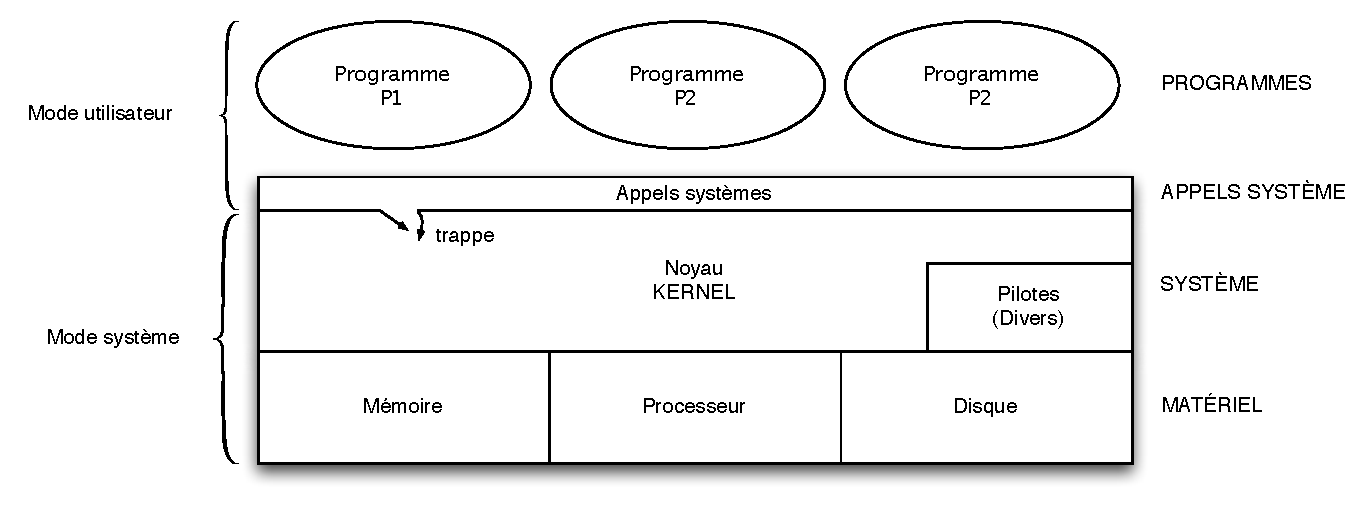
\includegraphics[scale=.75]{img/os}
\end{figure}

\subsection{Modes d'exécution} % (fold)
Il existe deux modes d'exécution : \begin{itemize}
	\item Mode utilisateur : accès restreint (confinement) aux ressources. Il s'agit de l'exécution des codes des programmes ;
	\item Mode système : accès privilégié à toutes les ressources du système (kernel + programmes utilisateurs). Il s'agit de l'exécution des codes du noyau.
\end{itemize}

Les \textbf{trappes} permettent le passage d'un mode à l'autre.

\subsection{Démarrage (boot)} % (fold)

L'allumage de l'ordinateur correspond à l'exécution d'un programme contenu dans la mémoire ROM (mémoire morte $\neq$ mémoire vive -- RAM) sur le CPU.

\begin{wrapfigure}{l}{0.17\textwidth}
  \vspace{-30pt}
  \begin{center}
    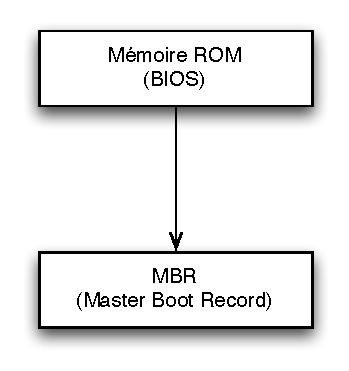
\includegraphics[width=0.15\textwidth]{img/boot}
  \end{center}
  \vspace{-45pt}
\end{wrapfigure}

Les différentes phases pour charger le système d'exploitation en mémoire :\begin{enumerate}
	\item Vérifier les périphériques ;
	\item Exécuter le premier bloc des disques (MBR) $\rightarrow$ \emph{Boot block} ;
	\item Charger le système d'exploitation.
\end{enumerate}

\vspace{10pt}

Multi-boot : remplacer le boot block par un programme fait un aiguillage (eg. GRUB, LILO\dots).
\begin{figure}[h!]
	\center
	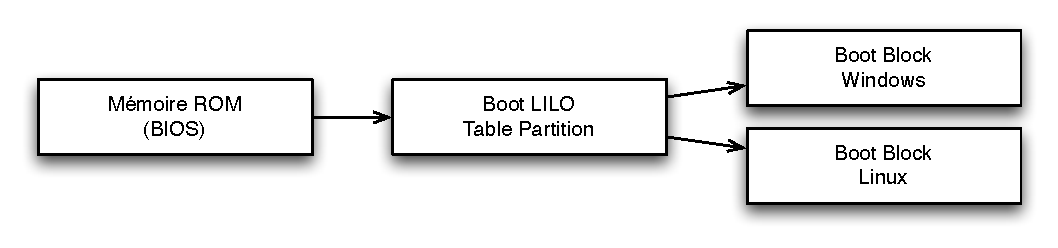
\includegraphics[scale=.5]{img/multi-boot}
	\vspace{-30pt}
\end{figure}

\chapter{Interruptions} % (fold)

\section{Introduction} % (fold)
\begin{def*}[Interruption]
	Une interruption (IT) est un signal généré par le \textbf{matériel} pour notifier un évènement au système d'exploitation.
	
	Le traitement des interruption est ensuite effectué par le système d'exploitation.
\end{def*}

\subsection*{Classification des interruptions} % (fold)
\begin{description}
	\item [Quand ?]\hfill\begin{enumerate}
		\item Évènement interne : lié à l'exécution du programme en cours
		\begin{ex*}
			Erreur de programmation (division par zéro, erreur d'adressage\dots).
		\end{ex*}
		\item Évènement externe : indépendant de l'exécution du programme en cours.
		\begin{ex*}
			Interruptions générées par des périphériques (contrôleur, clavier\dots) :\begin{itemize}
				\item Fin de transfert (contrôleur de disque) ;
				\item Horloge.
			\end{itemize}
		\end{ex*}
	\end{enumerate}
	\item[Types d'interruptions]\hfill \begin{enumerate}
		\item Interruptions liées aux entrées/sorties (\textbf{I}nput/\textbf{O}utput ou E/S) : transfert de données des périphériques vers la mémoire.\\
		$\rightarrow$ liés au contrôleur (Fin, Prêt, Erreur\dots).
		\item Interruptions externes\\
		$\rightarrow$ horloge, clavier\dots
		\item Appels système : interruptions/trappes générées explicitement par les programmes
		\item Déroutements : évènements interne, erreurs pendant l'exécution d'un programme.
		\item Erreurs matérielles
	\end{enumerate}
	\item[Priorités] propres à UNIX --- définies par le constructeur\hfill\\
		\begin{tabular}{rcl}
			+ prioritaire	& 0 & Horloge\\
			 				& 1 & Disque : I/O depuis le disque\\
			 				& 2 & Console (souris, clavier\dots)\\
			 				& 3 & Autres périphériques\\
			- prioritaire	& 4 & Appels  systèmes
		\end{tabular}
\end{description}

\section{Traitement d'interruptions} % (fold)
A chaque interruption, une commutation du mot d'état est automatiquement générée par le matériel.

État utilisateur $\overset{\mathrm{Trappe}}{\longrightarrow}$ État système

\begin{def*}[Mot d'état]
	Un mot d'état ou PSW (\emph{Processor Status Word}) représente :\begin{itemize}
		\item Etat du processeur (actif/inactif) ;
		\item Mode du processeur (utilisateur/système) ;
		\item Masque d'interruption ;
		\item PC/CO : compteur ordinal = la prochaine instruction à exécuter.
	\end{itemize}
\end{def*}

\begin{def*}[Vecteur d'interruptions]
	Un vecteur d'interruption est un tableau des adresses des fonctions liées à chaque interruptions prise en compte par le matériel. Les fonctions regroupent les routines d'interruption propre à chaque interruption.
\end{def*}

\begin{figure}[h!]
	\center
	\vspace{-15pt}
	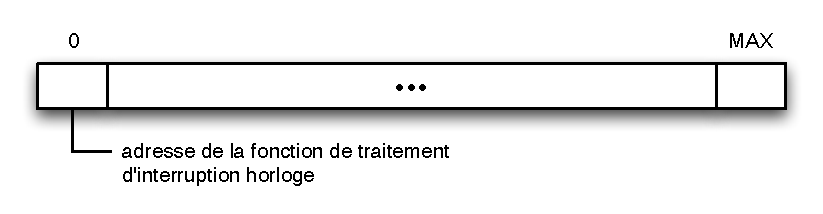
\includegraphics[scale=.6]{img/vecteur-interruptions}
	\vspace{-15pt}
\end{figure}


\begin{rem*}
	En général, les systèmes d'exploitation redéfinissent les fonctions du vecteur d'interruption.
\end{rem*}

\begin{figure}[h!]
	\center
	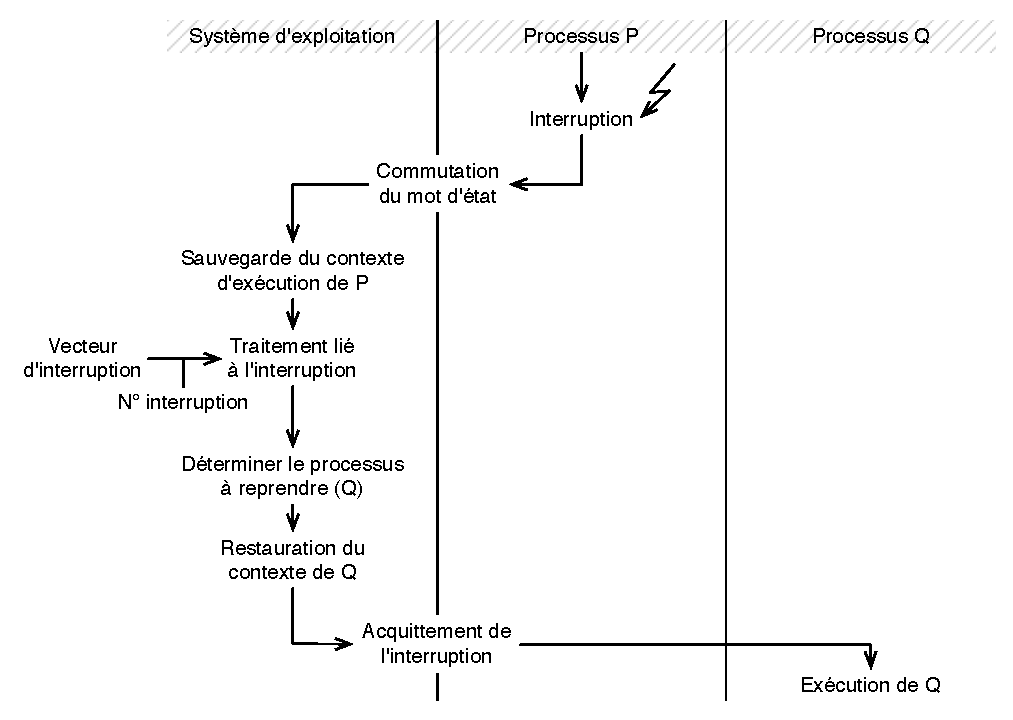
\includegraphics[scale=.6]{img/interruption}
	\vspace{-15pt}
\end{figure}

\section{Pile d'interruption} % (fold)
Des interruptions de priorité supérieure strictement peuvent survenir lors du traitement d'une interruption. Le système utilise une pile pour gérer les interruptions. La pile d'interruption permet un empilement de différentes interruptions.

\begin{figure}[h!]
	\center
	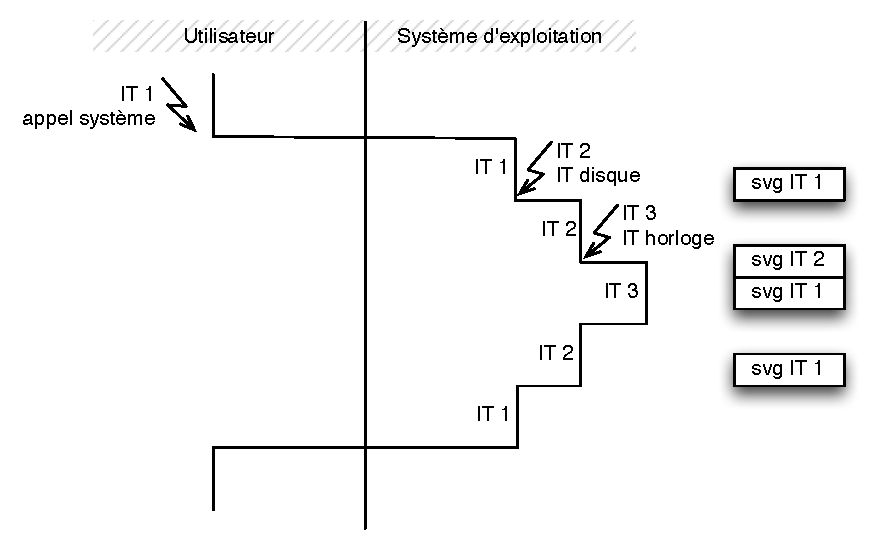
\includegraphics[scale=.6]{img/pile-interruptions}
	\vspace{-15pt}
\end{figure}

\section{Masquage/Désarmement d'interruption} % (fold)
\begin{def*}[Désarmement d'une interruption]
	C'est une \textbf{annulation} du traitement d'une interruption ou la prise en compte d'une interruption (eg. utile dans le cas d'un périphérique défaillant qui génère des interruptions inutiles).
\end{def*}

\begin{def*}[Masquage d'une interruption]
	Le masquage d'une interruption permet de \textbf{retarder} le traitement d'unes interruption.
	\begin{rem*}
		Le masquage d'une interruption permet de masquer toutes les interruptions de priorité inférieure ou égale à celle de l'interruption  masquée.
	\end{rem*}
\end{def*}

Pendant le traitement d'une interruption, les interruptions de priorité inférieure ou égale sont masquées.

La fonction de UNIX permettant de masquer une interruption est la fonction  SPL (\emph{Set Priority Level}).
\begin{figure}[h!]
	\center
	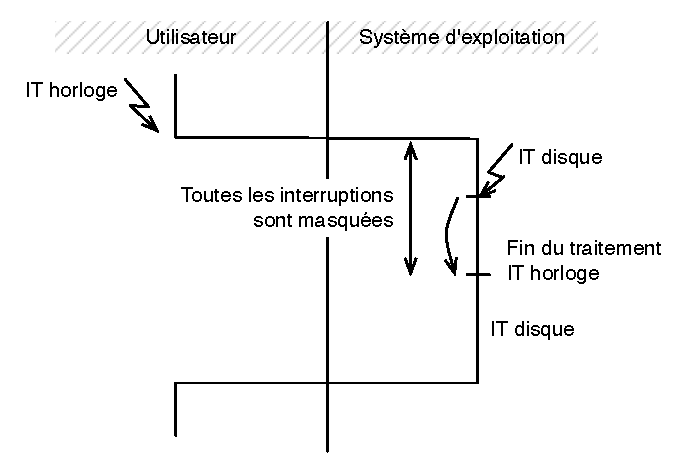
\includegraphics[scale=.6]{img/interruptions-masquees}
\end{figure}

\chapter{Ordonnancement} % (fold)
L'ordonnancement permet la gestion de l'accès des processus (tâches) au processeur.

\section{Introduction} % (fold)

Un algorithme d'ordonnancement (\emph{scheduling}) permet de choisir parmi un ensemble de tâches prêtes celle qui va occuper le processeur. Cet algorithme peut ou non utiliser des priorités affectées aux tâches.

\begin{def*}[Famine]
	La famine survient lorsque les critères utilisés par l'algorithme d'ordonnancement (alors inéquitable) pour déterminer la tâche élue sont tels que l'une des tâches n'est jamais choisie, et ne peut donc pas terminer son exécution. Un bon algorithme d'ordonnancement doit à tout prix éviter les problèmes de famine.
\end{def*}

Il existe deux modèles de programmation : \begin{itemize}
	\item Mono-programmation (\emph{monotask}) : un seul processus en mémoire $\Rightarrow$ pas d'ordonnancement.
	\item Multi-programmation (\emph{multitask}) : plusieurs processus en mémoire à un instant donné en concurrence pour l'accès au processeur.
\end{itemize}

\subsection{Types d'ordonnancement} % (fold)

\paragraph{Mode Batch} % (fold)
	La tâche élue conserve le processeur jusqu'à sa terminaison : elle ne peut être interrompue ni par l'arrivée d'une autre tâche, ni par une interruption horloge (eg. FCFS, SJN).\\
	Elle reste sur le processeur jusqu'à sa fin (mono-programmation) \textbf{ou} son blocage (eg. I/O : transfert sur/depuis le disque).
	\begin{figure}[h!]
		\center
		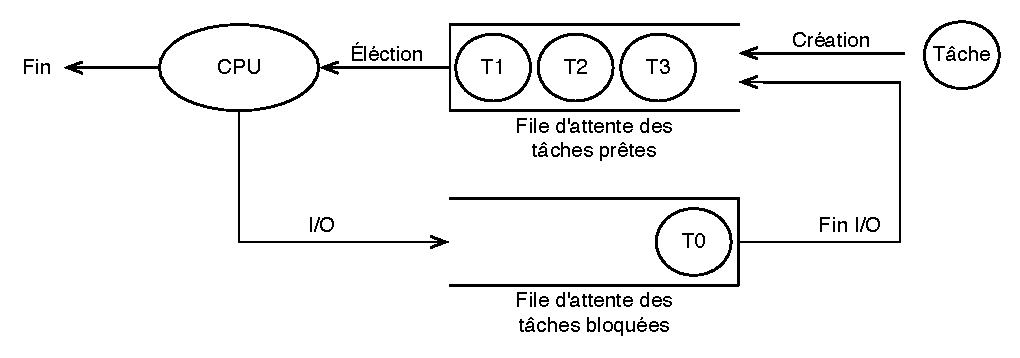
\includegraphics[scale=.75]{img/ordonnencement-batch}
	\end{figure}

\paragraph{Mode temps partagé} % (fold)
	Un \textbf{quantum} d'exécution correspond au temps maximal d'exécution continue d'une tâche (ie. sans interruption).
	\begin{rem*}
		Un quantum n'est pas une unité d'allocation de temps sur le processeur. Il s'agit d'une borne maximale du temps qu'un processus peut rester en continu sur le processeur. A la fin du quantum, le processus doit quitter le processeur et céder sa place à un autre processus.
	\end{rem*}
	\begin{figure}[h!]
		\center
		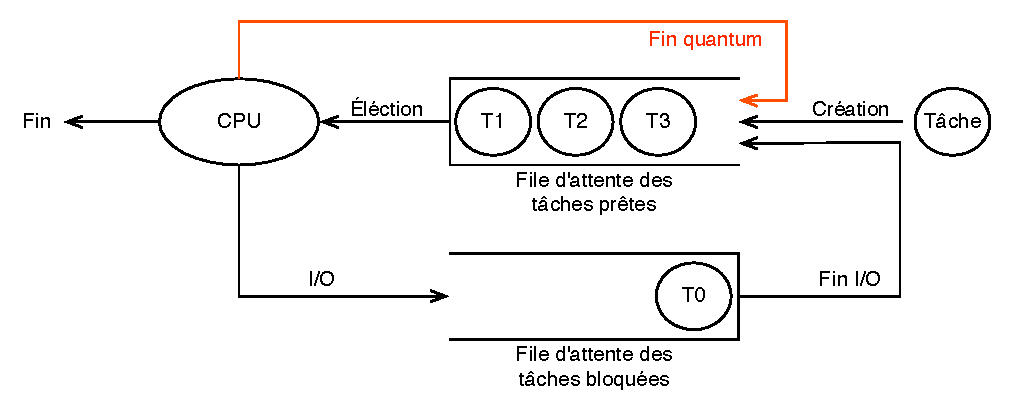
\includegraphics[scale=.75]{img/ordonnencement-split-time}
	\end{figure}


\subsection{Graphe d'état d'un processus} % (fold)

\begin{figure}[h]
  \centering
  \subfloat[Mode Batch]{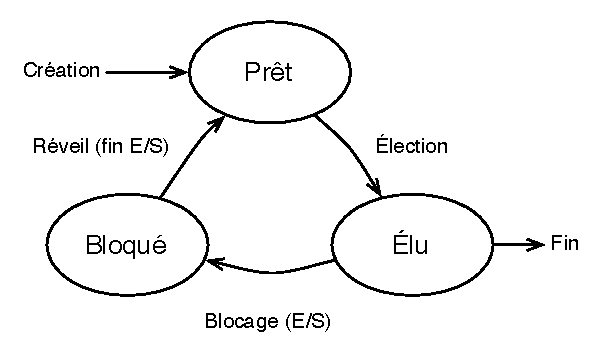
\includegraphics[width=0.47\textwidth]{img/etat-process-batch}}                
  \subfloat[Mode temps partagé]{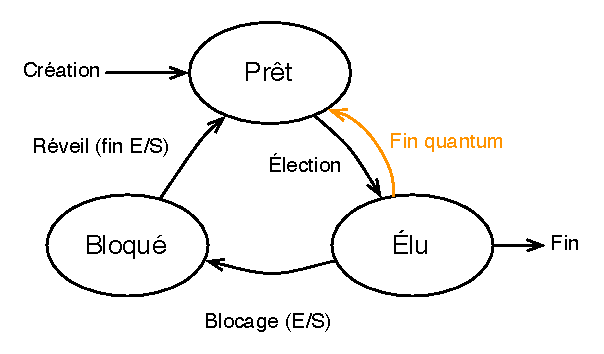
\includegraphics[width=0.47\textwidth]{img/etat-process-split-time}}
  \caption{Graphe d'état d'un processus}
\end{figure}

\subsection{Réquisition} % (fold)
\begin{def*}[Réquisition]
	Cela correspond à la possibilité pour une tâche plus prioritaire d'utiliser le processeur. Ainsi, seule l'arrivée d'une tâche plus prioritaire peut interrompre la tâche élue (eg. PSJN). La tâche élue est alors remise en tête de la file des tâches prêtes.
\end{def*}

Soient deux tâches T1, T2 telles que la priorité de T1 soit supérieure à celle de T2.

\begin{figure}[h!]
	\center
	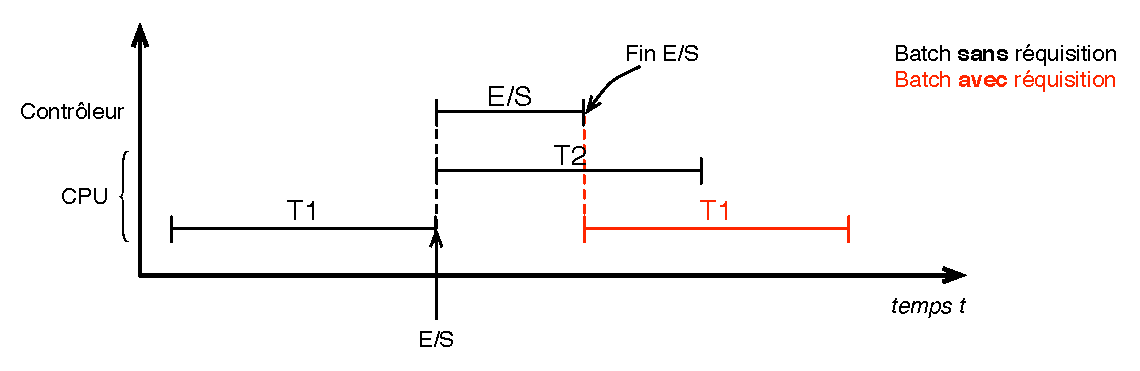
\includegraphics[scale=.65]{img/batch-requisition}
	\vspace{20pt}
\end{figure}

\section{Algorithmes d'ordonnancement -- mode Batch} % (fold)

\begin{rem*}
	On considérera un système sans quantum, avec ou sans réquisition.
\end{rem*}

\subsection{Premier arrivé, premier servi -- FIFO (\emph{First In, First Out}) ou FCFS (\emph{First Come, First Served})} % (fold)

\begin{ppe*}
	Les tâches sont traitées dans leur ordre d'arrivée.
\end{ppe*}

Considérons trois tâches T1, T2, T3 telles que :\begin{itemize}
	\item T1 est crée à $t=0$, de durée 24 secondes ;
	\item T2 est crée à $t=0$, de durée 3 secondes ;
	\item T3 est crée à $t=0$, de durée 3 secondes.
\end{itemize}

\begin{figure}[h!]
	\center
	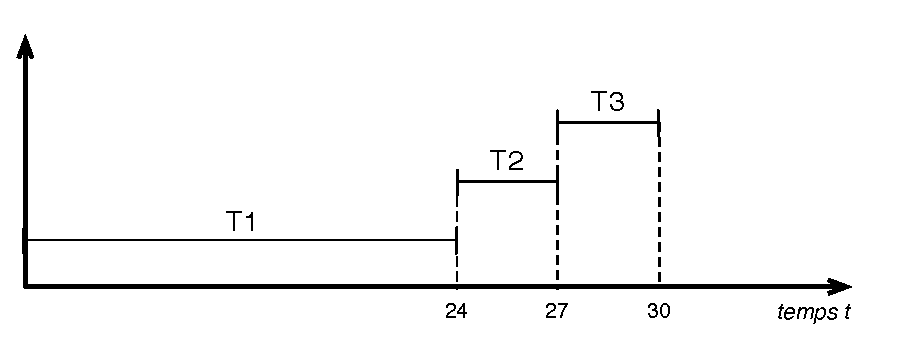
\includegraphics[scale=.65]{img/diagramme-gantt-batch}
\end{figure}


Tâches crées dans l'ordre : T1, T2, T3.

Calcul des différents temps de mesure pour une tâche :
\begin{itemize}
	\item Temps de réponse : $T_{r_{_{\mathrm{T}_{i}}}}=\textrm{date de fin de }\textrm{T}_{i}-\textrm{date de création de }\textrm{T}_{i}$ ;
	\item Temps d'attente : $T_{a_{_{\mathrm{T}_{i}}}}=\textrm{temps de réponse de }\textrm{T}_i - \textrm{durée de }\textrm{T}_i$.
\end{itemize}

\begin{tabularx}{\linewidth}{lXX}
	\toprule
	Tâche & Temps de réponse & Temps d'attente\tabularnewline
	\midrule
	\midrule
	T1 & $T_{r_{_{\mathrm{T}_{1}}}} = 24-0=24$ s & $T_{a_{_{\mathrm{T}_{1}}}} = 24-24=0$ s\tabularnewline
	\midrule
	T2 & $T_{r_{_{\mathrm{T}_{2}}}} = 27-0=27$ s & $T_{a_{_{\mathrm{T}_{2}}}} = 27-3=24$ s\tabularnewline
	\midrule
	T3 & $T_{r_{_{\mathrm{T}_{3}}}} = 30-0=30$ s & $T_{a_{_{\mathrm{T}_{3}}}} = 30-3=27$ s\tabularnewline
	\bottomrule
\end{tabularx}

Temps d'attente moyen : 17 secondes.

\subsection{Plus courts travaux d'abord -- SJF (\emph{Shortest Job First}) ou SJN (\emph{Shortest Job Next})} % (fold) 
\begin{ppe*}
	Le système choisit la tâche dont le temps d'exécution est le plus court (temps d'exécution de la tâche supposé connu).
\end{ppe*}

Considérons trois tâches T1, T2, T3 telles que :\begin{itemize}
	\item T1 est crée à $t=0$, de durée 24 secondes ;
	\item T2 est crée à $t=0$, de durée 3 secondes ;
	\item T3 est crée à $t=0$, de durée 3 secondes.
\end{itemize}

\begin{figure}[h!]
	\center
	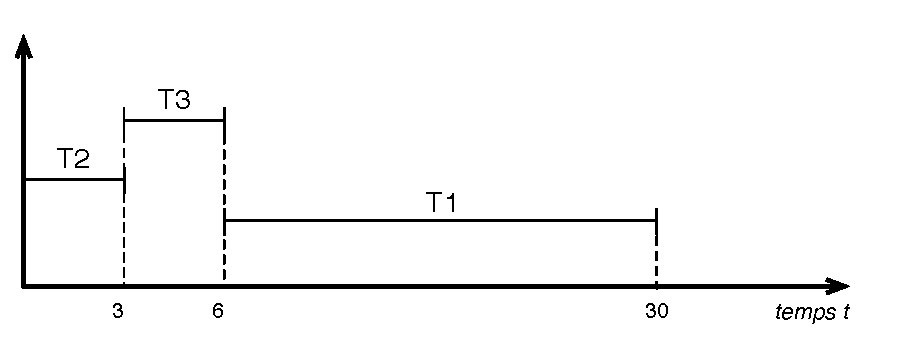
\includegraphics[scale=.65]{img/diagramme-gantt-batch-sjn}
\end{figure}

\begin{tabularx}{\linewidth}{lXX}
	\toprule
	Tâche & Temps de réponse & Temps d'attente\tabularnewline
	\midrule
	\midrule
	T1 & $T_{r_{_{\mathrm{T}_{1}}}} = 30-0=30$ s & $T_{a_{_{\mathrm{T}_{1}}}} = 30-24=6$ s\tabularnewline
	\midrule
	T2 & $T_{r_{_{\mathrm{T}_{2}}}} = 3-0=3$ s & $T_{a_{_{\mathrm{T}_{2}}}} = 3-3=0$ s\tabularnewline
	\midrule
	T3 & $T_{r_{_{\mathrm{T}_{3}}}} = 6-0=6$ s & $T_{a_{_{\mathrm{T}_{3}}}} = 6-3=3$ s\tabularnewline
	\bottomrule
\end{tabularx}

Temps d'attente moyen : 3 secondes.

\begin{ccl*}
	La stratégie SJF (\emph{Shortest Job First}) est meilleure que la stratégie FIFO (\emph{First In, First Out}).
	
	Quelques problèmes se posent :\begin{itemize}
		\item Le temps d'exécution est rarement connu à l'avance ;
		\item Risque de famine des tâches longues.
	\end{itemize}
\end{ccl*}

\section{Algorithmes à temps partagé} % (fold)

Utilisation de la notion de quantum (\emph{time-slice}).

\subsection{Implémentation} % (fold)

Implémentation d'algorithmes à temps partagé :\begin{itemize}
	\item Utilisation des registres horloge (RH et Rtempo) ;
	\item Utilisation d'un PIT (\emph{Programmable Interrupt Timer}).
\end{itemize}

\begin{def*}
	L'horloge (\emph{Timer}) est assimilable à un contrôleur. C'est un composant externe au processeur qui décrémente le registre horloge RH à une certaine fréquence (\textasciitilde 1MHz -- toues les $\mu$s).
	
	Si RH = 0, alors le Timer lève une interruption horloge, qui sera ensuite traitée par le système d'exploitation.
\end{def*}

Le Timer a pour rôle d'implémenter les quantum, mettre à jour l'heure de la machine, gérer les alarmes. 

Traitement d'une interruption horloge (interruption la plus prioritaire du système) :\begin{itemize}
	\item Traiter les alarmes ;
	\item Mise à jour de l'horloge ;
	\item Elire un nouvelle tâche ;
	\item Réinitialiser le registre RH.
\end{itemize}

\begin{rem*}
	Le registre RH est un registre privilégié.
\end{rem*}

\begin{figure}[h!]
	\center
	\vspace{-20pt}
	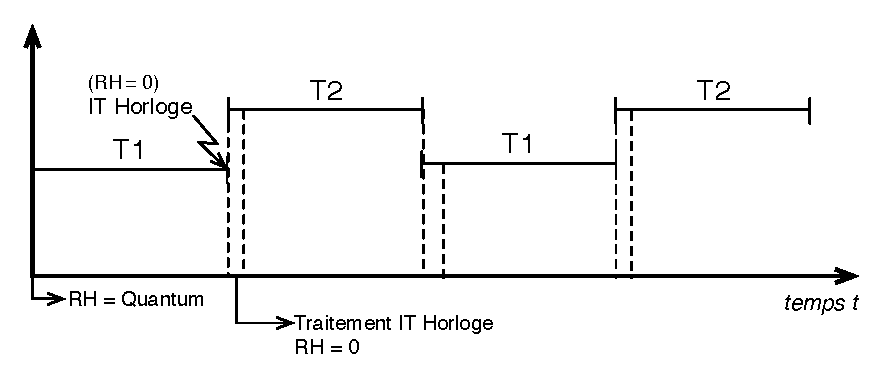
\includegraphics[scale=.65]{img/IT-Horloge}
	\vspace{-20pt}
\end{figure}

Le quantum est lié à la perception de parallélisme de l'utilisateur. de ce fait, le quantum a une durée d'environ 100 ms.

\begin{def*}[Tick]
	Un Tick (ou \emph{jiffies} au sens de Linux) est la valeur (temps) entre deux interruptions horloge. Un tick est un paramètre système initialisé à environ 1 -- 10 ms.
	\[\textrm{Quantum} = N\times \textrm{Tick}\]
\end{def*}
\begin{figure}[h!]
	\center
	\vspace{-30pt}
	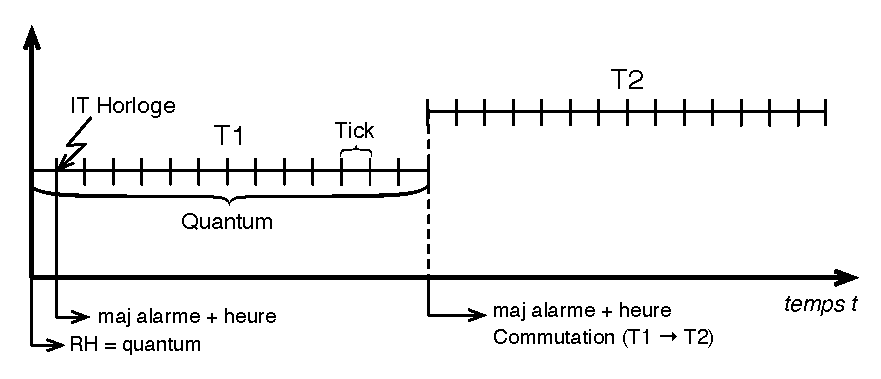
\includegraphics[scale=.65]{img/tick-quantum}
	\vspace{-20pt}
\end{figure}

Une expiration de quantum aura ainsi lieu tous les $N$ ticks.

\subsection{Algorithme du tourniquet -- RR (\emph{Round Robbin})} % (fold)
Accès des tâches à tour de rôle au processeur. Cet algorithme nécessite une file des tâches prêtes.

\begin{description}
	\item [Création d'une tâche] Insertion en queue ;
	\item [Election d'une tâche] ($N$ ticks) Choisir la tâche en tête de la file des tâches prêtes ;
	\item [Fin de quantum] ($N$ ticks) Réinsertion de la tâche élue en queue. Celle-ci devient une tâche prête.
\end{description}

Soient trois tâches T1, T2, T3 créées dans cet ordre à $t=0$ : \begin{itemize}
	\item T1 dure 200 ms;
	\item T2 dure 30 ms;
	\item T3 dure 100 ms.
\end{itemize}
Considérons un quantum de durée 40 ms et un temps de commutation négligeable ($<1$ ms).

\begin{figure}[h!]
	\center
	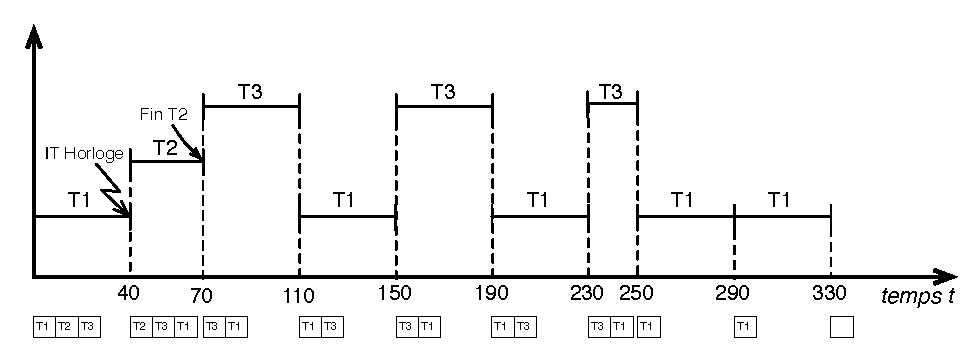
\includegraphics[scale=.65]{img/round-robbin}
\end{figure}

Temps d'attente des différentes tâches :\begin{itemize}
	\item $T_{a_{_{\mathrm{T}_{1}}}} = (330-0)-200=130$ ms;
	\item $T_{a_{_{\mathrm{T}_{2}}}} = (70-0)-30=40$ ms;
	\item $T_{a_{_{\mathrm{T}_{3}}}} = (250-0)-100=150$ ms;
\end{itemize}

Lors d'une entrée / sortie, la tâche passe à l'état bloqué. A la fin de l'E/S, la tâche passe à l'état prêt.\\
Il faudrait alors donner une priorité plus forte aux tâches réveillées (ie. qui sortent de l'état bloqué) en maintenant la position de la tâche dans la file. Au réveil de la tâche, le quantum restant de celle-ci lui est alloué.

\begin{ex*}
	Soit la file des tâches suivante (P : état prêt, B : état bloqué) : 
	\begin{figure}[h!]
		\center
		\vspace{-10pt}
		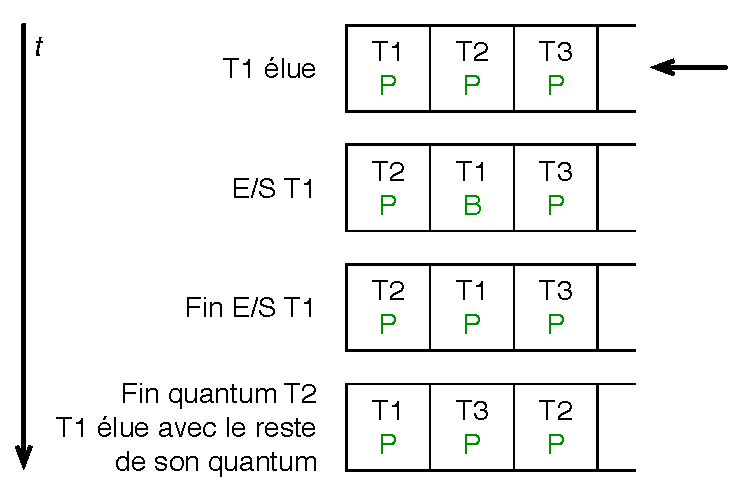
\includegraphics[scale=.50]{img/FIFO}
		\vspace{-10pt}
	\end{figure}
\end{ex*}

Avantages / inconvénients de cet ordonnancement :\begin{itemize}
	\Pitem Equitable, simple ;
	\Pitem Pas de famine : si une tâche $T$ est prête, soit $n$ la taille de la file devant $T$ et $q$ la quantum, alors $T$ attend $n\times q$ ;
	\Citem Trop équitable : pas de priorités entre les tâches.
\end{itemize}

\subsection{Priorités} % (fold)
\subsubsection{Priorité fixe (statique)} % (fold)
Chaque tâche dispose à sa création d'une priorité qui conserve la même valeur tout au long de son exécution.

Considérons une priorité fixe avec $N$ niveaux de priorités et une file par niveau de priorité.

\begin{description}
	\item[Création d'une tâche] Attribuer un niveau à la tâche, insertion de celle-ci en queue de la file correspondante.
	\item[Election d'une tâche] Choisir la tâche prête de la file non vide la plus prioritaire.
	\item[Fin du quantum] La tâche élue est ré-insérée en queue de sa file.
\end{description}

\begin{figure}[h!]
	\center
	\vspace{-10pt}
	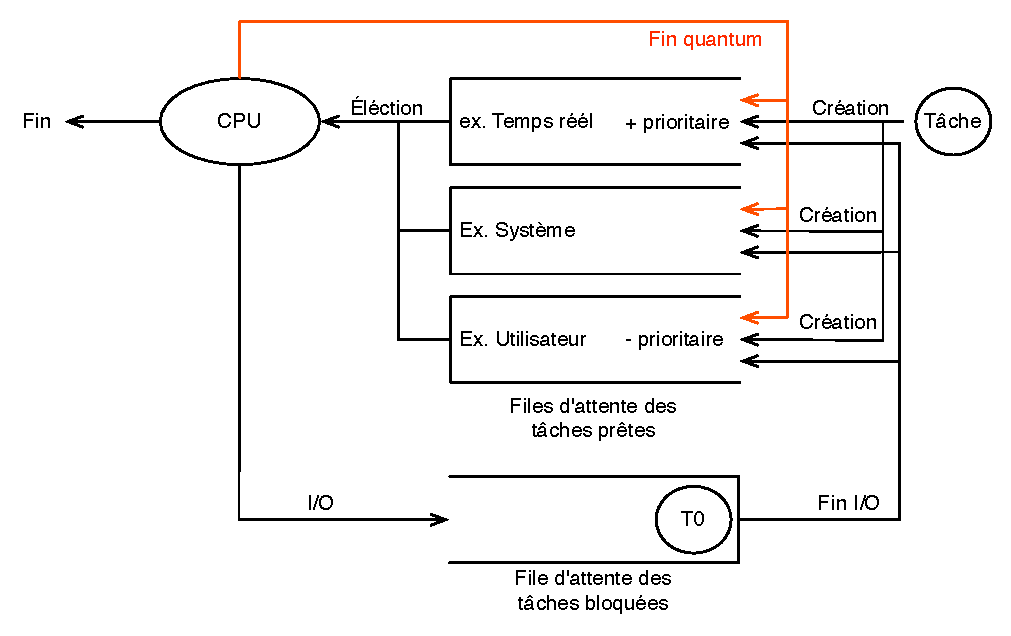
\includegraphics[scale=.65]{img/priorite-fixe}
	\vspace{-10pt}
\end{figure}

Avantages / inconvénients de cet ordonnancement :\begin{itemize}
	\Pitem Permet de prendre en compte les tâches prioritaires ;
	\Citem Pas équitable : risque de famine des tâches les moins prioritaires.
\end{itemize}

\subsubsection{Priorité dynamique} % (fold)
Les priorités affectées aux tâches changent en cours d'exécution. Plusieurs algorithme sont alors possibles suivant le critère de changement de priorité.

Considérons une priorité dynamique avec $N$ files de $F_0$ à $F_{N-1}$ (où la file $F_0$ est la plus prioritaire).

\begin{description}
	\item[Création d'une tâche] Insertion de la tâche en queue de la file $F_0$.
	\item[Election d'une tâche] Choisir la tâche prête de la file non vide la plus prioritaire (utilisation d'une boucle d'attente \lstinline!while!).
	\item[Fin quantum] La tâche élue est ré-insérée en queue de la \textbf{file suivante}.
\end{description}

\begin{rem*}
	Les tâches issues de la file $F_{N-1}$ sont ré-insérées en queue de la file $F_0$.
\end{rem*}

\begin{figure}[h!]
	\center
	\vspace{-10pt}
	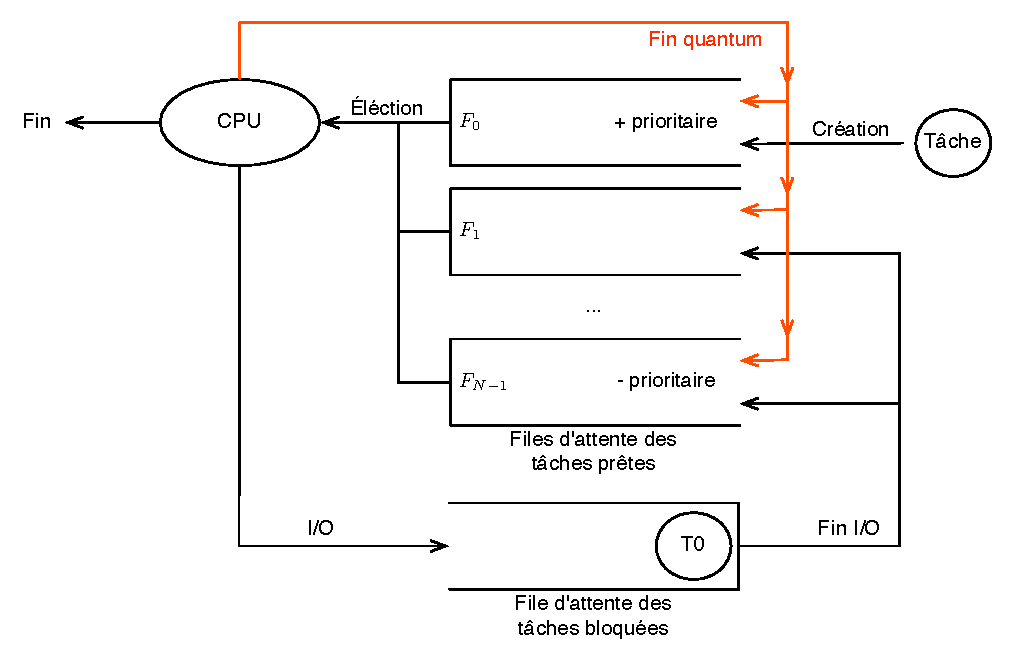
\includegraphics[scale=.65]{img/priorite-dynamique}
	\vspace{-10pt}
\end{figure}

Avantages / inconvénients de la priorité dynamique :\begin{itemize}
	\Pitem \textbf{Plus} une tâche est élue, \textbf{moins} elle est prioritaire.
	\Pitem Une tâche ancienne est donc moins prioritaire ;
	\Pitem Approximation de SJF (\emph{Shortest Job First}) sans connaître à l'avance la durée des tâches.
	\Citem Risque de famine des tâches longues si il y a un flot continu de création de tâches.
	\Citem Résolution de la famine : régulièrement (tous les $N$ quantum \textasciitilde 1 seconde), le système remonte la priorité des toutes les tâches prêtes.
\end{itemize}

\section{Ordonnancement dans les systèmes ``modernes''} % (fold)
\begin{figure}[h!]
	\center
	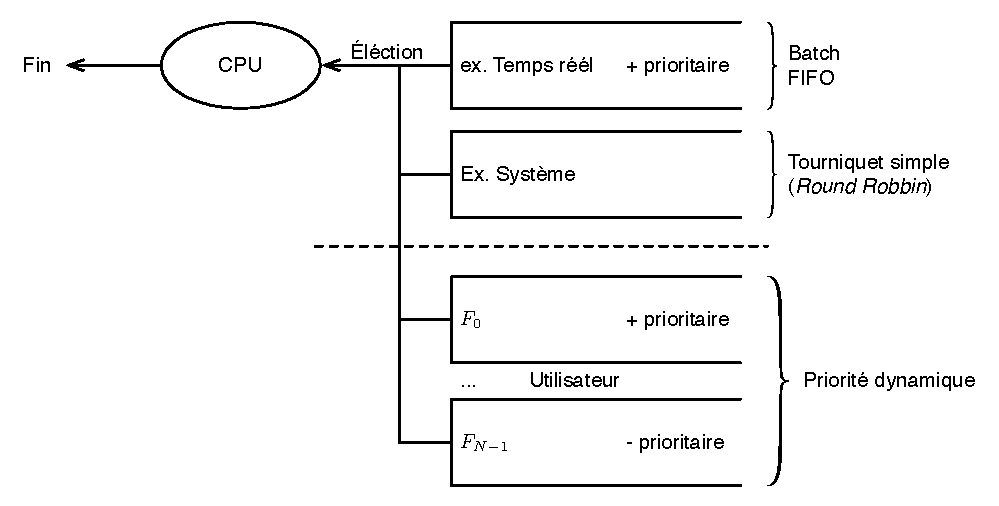
\includegraphics[scale=.65]{img/systeme-moderne}
	\vspace{-20pt}
\end{figure}

\chapter{Processus UNIX} % (fold)
\section{Introduction} % (fold)

Un processus en mémoire correspond à :\begin{itemize}
	\item Une pile (variables locales) -- R/W ;
	\item Un segment données (variables globales, tas) -- R/W ;
	\item Un code -- R.
\end{itemize}


Contexte matériel du processus : registres.

Informations système :\begin{itemize}
	\item pid : numéro de processus (unique) ;
	\item uid : numéro d'utilisateur ayant exécuté le processus ;
	\item gid : numéro du groupe auquel appartient l'utilisateur ayant lancé le processus.
\end{itemize}

Le système contient une table globale regroupant tous les processus : \lstinline!proc[]! ou \lstinline!task[]!.
\begin{figure}[h!]
	\center
	\vspace{-10pt}
	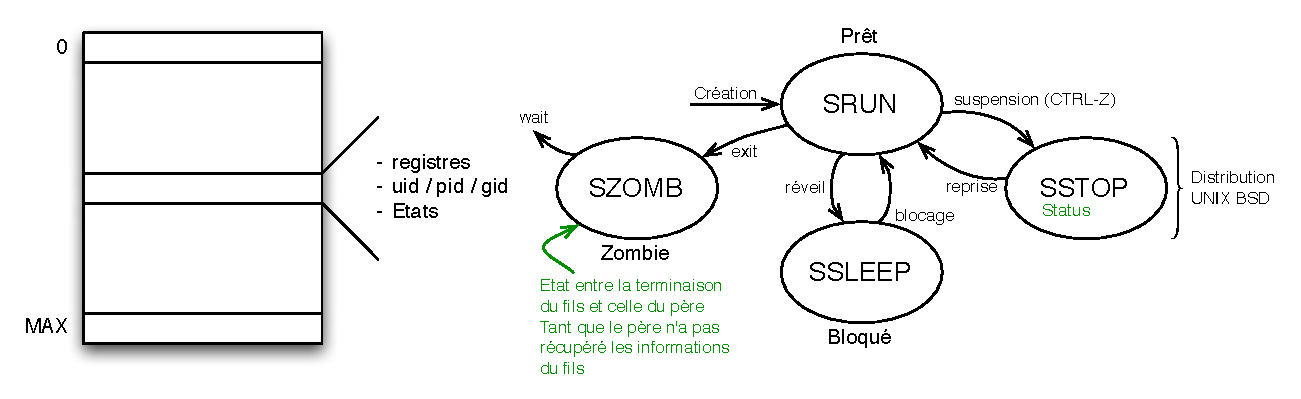
\includegraphics[scale=.65]{img/processus-UNIX}
	\vspace{-20pt}
\end{figure}

\section{Primitives permettant de manipuler les processus} % (fold)
Afin de savoir quels sont les directives pré-processeur \lstinline!#include! à utiliser, s'informer avec la commande \lstinline!man <commande>! du terminal.

En général, utiliser :
\begin{lstlisting}
#include <unistd.h>
#include <stdlib.h>
#include <stdio.h>
\end{lstlisting}

\subsection{Création d'un processus} % (fold)
\begin{figure}[h!]
	\center
	\vspace{-10pt}
	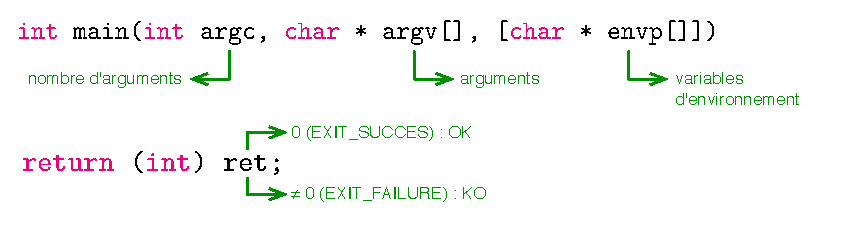
\includegraphics[scale=.75]{img/main}
\end{figure}

Soit l'exécutable \lstinline!./mon_prog! créé à la suite de la compilation. On a alors :

\begin{tabular}{cccccc}
	\lstinline!argv[0]! & \lstinline!argv[1]! & \lstinline!argv[2]! & \dots & \lstinline!argv[argc-1]! & \lstinline!argv[argc]!\\
	\lstinline!./mon_prog! & \lstinline!arg1! & \lstinline!arg2! & \dots & \lstinline!argN! & \lstinline!NULL!\\
\end{tabular}

\subsection{Création de nouveaux processus} % (fold)
Notion de filiation :
\begin{figure}[h!]
	\center
	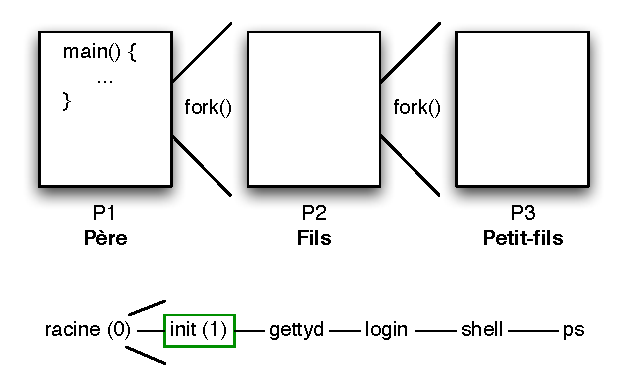
\includegraphics[scale=.75]{img/fork1}
\end{figure}

Primitive (appel système) \lstinline!pid_t fork();! création par duplication du père

\begin{rem*}
	Le type \lstinline!pid_t! est assimilable au type \lstinline!int!.\\
	Il n'y a pas de partage de variables une fois le processus père dupliqué.
\end{rem*}

\begin{figure}[h!]
	\center
	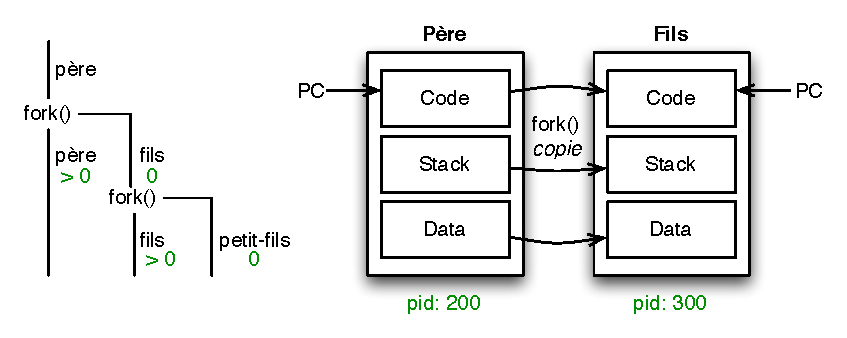
\includegraphics[scale=.75]{img/fork2}
\end{figure}

La valeur de retour de \lstinline!fork()! permet de distinguer le processus père du processus fils créé : \begin{itemize}
	\item $>0$ : pid du processus fils ; valeur retournée au processus père ;
	\item 0 : valeur retournée au processus fils (pour savoir son pid : \lstinline!pid_t getpid()!) ;
	\item -1 : erreur sur la fonction \lstinline!fork()! (la table des processus est probablement remplie).
\end{itemize}

Il existe également d'autres primitives relatives aux processus :\begin{itemize}
	\item \lstinline!pid_t getpid(void)! : retourne le pid du processus courant ;
	\item \lstinline!pid_t getppid(void)! : retourne le pi du père (parent) du processus courant.
\end{itemize}

\begin{ex*}
	Soit le code suivant :
\begin{lstlisting}
int main(int argc, char * argv[]) {
	pid_t p;
	int a = 10;
	p = fork();
	
	if(p == -1) { // Erreur
		perror("Erreur sur le fork.\n");
		return 1;
	}
	
	if(p == 0) { /* le fils */
		printf("Je suis le fils %d, pere : %d.\n", getpid(), getppid());
		a++;
		return 0; // a = 11
	} else { /* le pere */
		printf("Pere de %d.\n", p);
		return 0; // a = 10
	}
}
\end{lstlisting}	
\end{ex*}

\subsection{Terminaison} % (fold)

La terminaison d'un processus s'effectue avec la primitive \lstinline!void exit(int etat);!

Le processus se termine en retournant la valeur entière \lstinline!etat!. Il passe alors à l'état \emph{zombie} jusqu'à ce que son père récupère son état de sortie (à l'aide de la primitive \lstinline!wait(&status)!).

\begin{rem*}
	Les valeurs \lstinline!EXIT_SUCCESS! (0) et \lstinline!EXIT_FAILURE! ($\neq 0$) sont définies avec le C Standard (ISO C99).
\end{rem*}

\subsection{Recouvrement (primitive exec)} % (fold)

\begin{def*}[Recouvrement]
	Le recouvrement permet à un processus de changer (écraser) sont code. De ce fait, le processus va exécuter un nouveau \lstinline!main!.
\end{def*}

\begin{rem*}
	Le recouvrement ne permet pas de créer de nouveau processus. En effet, le processus garde le même pid et le même père.\\
	Pour créer un nouveau processus : \lstinline!fork()! puis \lstinline!exec()!.
\end{rem*}

\paragraph{Primitives} % (fold)

Les différentes primitives de recouvrement (\lstinline!exec!) sont présentées dans la suite.

\begin{figure}[h!]
	\center
	\vspace{-20pt}
	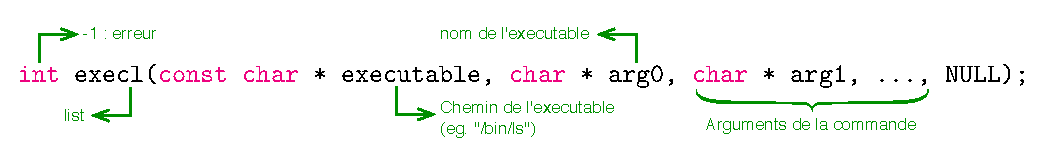
\includegraphics[scale=.75]{img/execl}
	\vspace{-10pt}
\end{figure}

\begin{ex*}
	Soit le code suivant :
\begin{lstlisting}
p = fork();
if(p == -1) { // Erreur
	perror("Erreur sur le fork.\n");
	return 1;
}
if(p == 0){ /* le fils */
	execl("/bin/ls", "ls", "f1", NULL);
	perror("lb exec");
	exit(1);
}
\end{lstlisting}
\end{ex*}

\begin{figure}[h!]
	\center
	\vspace{-20pt}
	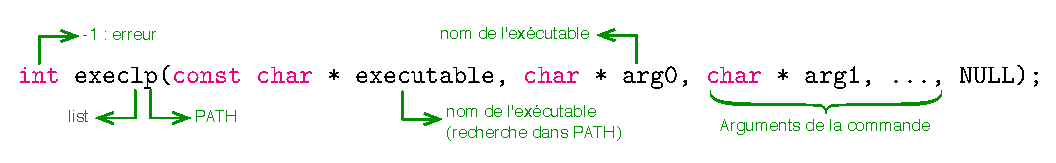
\includegraphics[scale=.75]{img/execlp}
	\vspace{-10pt}
\end{figure}

\begin{ex*}
	\lstinline!execlp("ls", "ls", "f1", NULL);!
\end{ex*}

\begin{figure}[h!]
	\center
	\vspace{-20pt}
	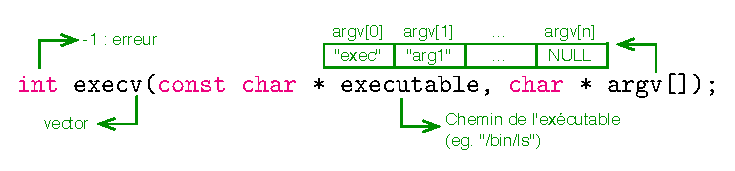
\includegraphics[scale=.75]{img/execv}
	\vspace{-10pt}
\end{figure}

\begin{ex*}
	Soit le code suivant :
\begin{lstlisting}
char * argv[3] = {"ls", "f1", NULL};
execv("/bin/ls", argv);
\end{lstlisting}
\end{ex*}

\begin{figure}[h!]
	\center
	\vspace{-20pt}
	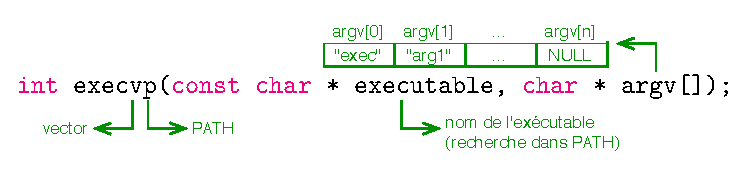
\includegraphics[scale=.75]{img/execvp}
	\vspace{-10pt}
\end{figure}

\begin{ex*}
	Soit le code suivant :
\begin{lstlisting}
char * argv[3] = {"ls", "f1", NULL};
execvp("ls", argv);
\end{lstlisting}
\end{ex*}

\begin{rem*}
	Il existe également les primitives \lstinline!execle! et \lstinline!execve! qui permettent aussi de modifier les variables d'environnement du processus à exécuter.
\end{rem*}

\subsection{Synchronisation père/fils ( primitive wait)}

La primitive \lstinline!pid_t wait(int * etat)! permet au père d'attendre la fin d'un seul fils quelconque.

\begin{rem*}
	S'il faut attendre la fin de $n$ fils, il faut faire une boucle \lstinline!for! contenant $n$ itérations appelant à chaque fois la primitive \lstinline!wait!. En général, il faut autant de \lstinline!wait! que de \lstinline!fork!.
	
	L'argument \lstinline!etat! passé par référence à la primitive \lstinline!wait! n'est pas forcément alloué dynamiquement (avec \lstinline!malloc!). Il est possible de l'allouer statiquement, puis de le passer par référence.
\end{rem*}

\begin{figure}[h!]
	\center
	\vspace{-20pt}
	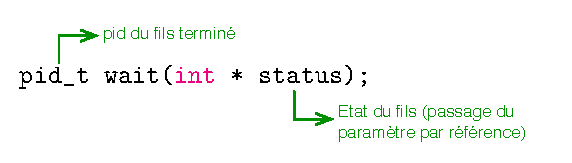
\includegraphics[scale=.75]{img/wait}
	\vspace{-10pt}
\end{figure}
Argument et valeur de retour :\begin{itemize}
	\item Valeur de retour : pid du processus fils terminé ;
	\item Paramètre de sortie \lstinline!status! passé par référence : état du processus fils (valeur de retour de \lstinline!exit!).
\end{itemize}

Marcos définies dans \lstinline!<wait.h>! manipulant le paramètre \lstinline!etat! :\begin{itemize}
	\item \lstinline!WEXITSTATUS(status)! : valeur de retour ;
	\item \lstinline!WIFEXITED(status)! : valeur $\neq 0$ si fin normale.
\end{itemize} 

\begin{ex*}
	Soit le code suivant :
\begin{lstlisting}
pid_t p, d;
int e;
p = fork();
if(p == -1) { // Erreur
	perror("Erreur sur le fork.\n");
	return 1;
}

if(p == 0){	/* le fils */
	exit(2);
} else { /* le pere */	
	d = wait(&e); // wait(NULL) -- pere bloque
	if(WIFEXITED(e)){ // WEXITSTATUS(e) == 0
		printf("Fin normale de %d.\n", d);
	} else {
		printf("Probleme fils : %d, etat : %d.\n", d, WEXITSTATUS(e));
	}
}
\end{lstlisting}
\end{ex*}

\begin{rem*}
	La primitive \lstinline!wait! retourne -1 si pas de fils.
	
	Le fils terminé reste à l'état de zombie jusqu'à ce que le père fasse \lstinline!wait!.
\end{rem*}

\begin{ex*}
	Créer un zombie pendant 30 secondes (environ)
\begin{lstlisting}
p = fork();
if(p == -1) { // Erreur
	perror("Erreur sur le fork.\n");
	return 1;
}

if(p == 0){ /* le fils */
	exit(0);
} else { /* le pere */
	sleep(30);
	wait(NULL);
}
\end{lstlisting}
\end{ex*}	 

\begin{rem*}
Si le père est terminé, ses fils (orphelins) sont ``adoptés'' par `\lstinline!init! (processus fils du processus racine dont le pid est égal à 1).
\end{rem*}

\begin{figure}[h!]
	\center
	\vspace{-20pt}
	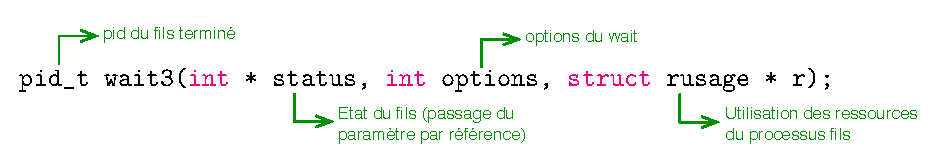
\includegraphics[scale=.75]{img/wait3}
	\vspace{-10pt}
\end{figure} 
Arguments :\begin{itemize}
	\item \lstinline!options! :\begin{itemize}
		\item 0 pas d'option ;
		\item \lstinline!WNOHANG!, non bloquant retourne 0 si fils pas terminé.
	\end{itemize} 
	\item Structure \lstinline!struct rusage! (\lstinline!man getrusage!) :
\begin{lstlisting}
struct rusage {
	struct timeval ru_utime; /* CPU consomme par le fils en mode user */
	strcut timeval ru_stime; /* CPU consomme par le fils en mode system */
}
\end{lstlisting}
\end{itemize}

\begin{figure}[h!]
	\center
	\vspace{-20pt}
	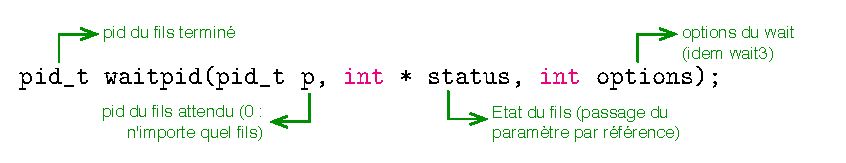
\includegraphics[scale=.75]{img/waitpid}
	\vspace{-10pt}
\end{figure}
Arguments :\begin{itemize}
	\item \lstinline!p! : pid du fils attendu (0 : n'importe quel fils) ;
	\item \lstinline!options! : idem que \lstinline!wait3!.
\end{itemize}

\chapter{Synchronisation entre tâches}

\section{Définitions}
On considère un système:
\begin{itemize}
	\item Multi-programmation (multi-tâches) en temps partagé ;
	\item Plusieurs tâches partagent des données (variables).
\end{itemize}

\begin{figure}[h!]
	\center
	\vspace{-10pt}
	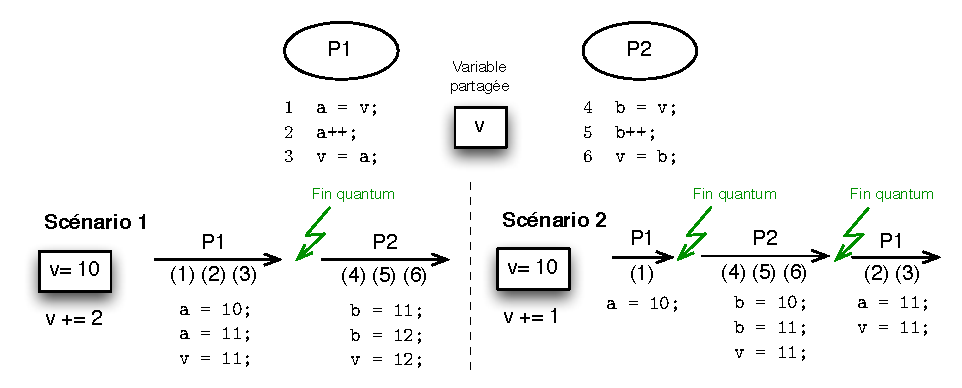
\includegraphics[scale=1]{img/partage-variable}
	\vspace{-10pt}
\end{figure}

On a alors affaire à un code non déterministe (plusieurs issues différentes non prévisibles).

\begin{def*}[Ressource critique]
	Une ressource critique est une ressource partagée entre plusieurs processus et dont l'accès doit être contrôlé pour préserver la cohérence de son contenu (variable \lstinline!v!, fichier, etc.). En particulier, ce contrôle peut impliquer un accès en exclusion mutuelle, c'est-à-dire que la ressource n'est jamais accédée par plus d'un processus à la fois.
\end{def*}

\begin{def*}[Sections critiques -- SC]
	Les sections critiques sont des portions de codes manipulant des ressources critiques (dans le cas de l'exemple, il s'agit des sections (1)(2)(3) et (4)(5)(6)). Ces portions de code doivent être exécutée de manière indivisible.
\end{def*}

\begin{def*}[Indivisibilité]
	L'indivisibilité signifie que deux sections critiques concernant une même ressource ne sont jamais exécutées simultanément mais toujours séquentiellement (dans un ordre arbitraire). Il y a ainsi exclusivité entre ces séquences d'instructions.
\end{def*}

\begin{def*}[Exclusion mutuelle]
	L'exclusion mutuelle est le mécanisme qui assure qu'un processus au plus est en section critique sur une même variable.
\end{def*}

\begin{def*}[Synchronisation]
	L'exclusion mutuelle n'est qu'un cas particulier de synchronisation. Une synchronisation est une opération influant sur l'avancement d'un ensemble de processus :\begin{itemize}
		\item Etablissement d'un ordre d'occurrence pour certaines opérations (envoyer / recevoir) ;
		\item Respect d'une condition (rendez-vous, exclusion mutuelle, etc.).
	\end{itemize}
\end{def*}

\begin{def*}[Attente active]
	L'attente active est la mobilisation d'un processeur pour l'exécution répétitive d'une primitive de synchronisation jusqu'à ce que la condition de synchronisation permette la continuation normale du processus.
\end{def*}

\begin{def*}[Interblocage (\emph{deadlock})]
	L'interblocage se produit lorsque deux processus concurrents s'attendent mutuellement. Les processus bloqués dans cet état le sont alors définitivement.
\end{def*}

\section{Mécanisme d'exclusion mutuelle}
Propriétés des algorithmes d'exclusion mutuelle :
\begin{itemize}
	\item Sûreté : un processus au plus en section critique ;
	\item Vivacité : toutes les demandes d'accès aux sections critiques doivent être satisfaites.
\end{itemize}

\begin{figure}[h!]
	\center
	\vspace{-10pt}
	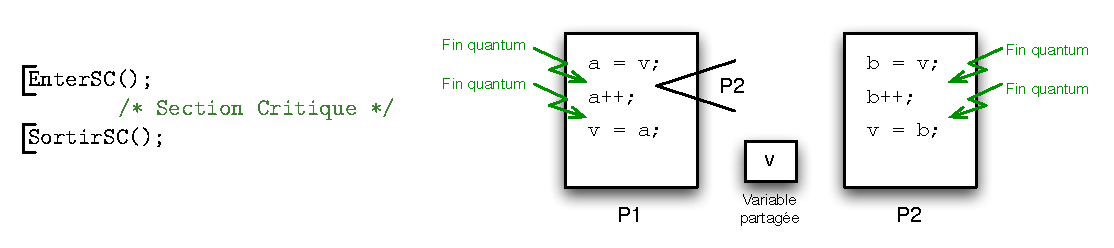
\includegraphics[scale=.85]{img/SC}
	\vspace{-10pt}
\end{figure}

Les primitives \lstinline!EntrerSC()! et \lstinline!SortirSC()! doivent être rendues indivisibles (opérations atomiques) pour garder la cohérence de leur contenu. De ce fait, il faut masquer les interruptions système pendant leur exécution et les rendre primitives système.

\subsection{Masquage IT Horloge}
Le masquage de l'interruption horloge permet de désactiver le temps partagé pendant la section critique : \begin{itemize}
	\item \lstinline!EntrerSC()! : Masque l'IT Horloge ;
	\item \lstinline!SortirSC()! : Démasquer l'IT Horloge.
\end{itemize}

Plusieurs problèmes se posent alors :
\begin{itemize}
	\item Trop dangereux -- risque de monopoliser le processeur ;
	\item Exclut \textbf{tous} les processus ;
	\item Le masque d'IT Horloge est utilisé en interne par le système.
\end{itemize}

\subsection{Variables de synchronisation}
Des variables partagées indiquent si les ressources critiques sont disponibles.

\subsubsection{Solution 1. Une variable booléenne}
Soit la variable \lstinline!bool lock! ayant pour valeur :\begin{itemize}
	\item \lstinline!true! si la ressource est verrouillée ;
	\item \lstinline!false! si la ressource est non verrouillée.
\end{itemize}

\begin{figure}[h!]
	\center
	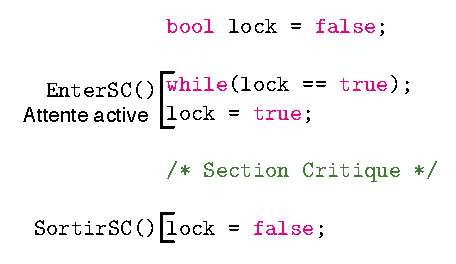
\includegraphics[scale=.85]{img/SC-bool}
\end{figure}

\begin{figure}[h!]
	\center
	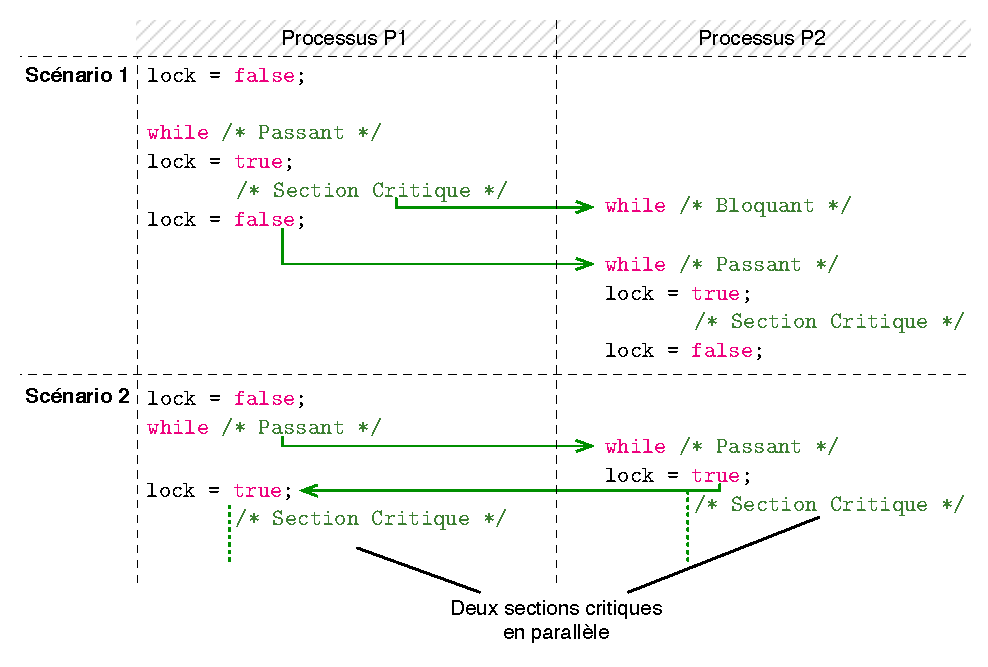
\includegraphics[scale=.85]{img/SC-bool-scenario}
\end{figure}


\subsubsection{Solution 2. Algorithme de Peterson (1981)}
L'algorithme de Peterson assure l'exclusion mutuelle pour deux processus $P_i$ et $P_j$ (généralisable). Cet algorithme est basé sur l'attente active des deux processus $P_i$ et $P_j$.

Soient les variables partagées : 
\begin{itemize}
\item Un tableau de booléen \lstinline!flag! indique si un processus est demandeur de section critique (SC) ;
\item Une variable \lstinline!tour! indique à qui le tour.
\end{itemize}

\begin{figure}[h!]
	\center
	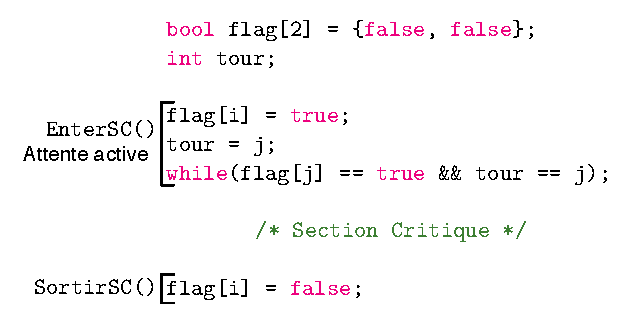
\includegraphics[scale=.85]{img/SC-peterson}
\end{figure}

\begin{description}
	\item[Cas 1] Le processus $P_i$ demande seul l'accès à la section critique.\\
	\lstinline!flag[j] == false! et \lstinline!while! passant.\\
	Le processus $P_i$ a accès à la section critique.
	\item[Cas 2] Les processus $P_i$ et $P_j$ demandent l'accès à la section critique.\\
	La variable \lstinline!tour! fixe l'ordre.
\end{description}
\clearpage
\begin{figure}[h!]
	\center
	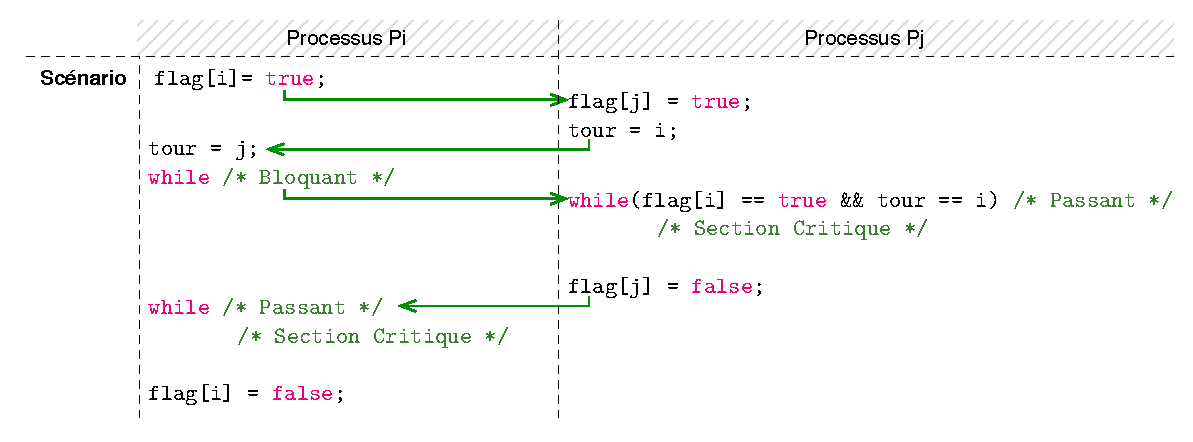
\includegraphics[scale=.85]{img/SC-peterson-scenario}
\end{figure}


\subsubsection{Solution 3. Test-and-set (t-a-s)}
\begin{def*}[Test-and-set]
	Un bloc d'instructions indivisible pour positionner et tester une variable. Il ne peut pas y avoir d'interruption pendant l'exécution du code de test-and-set.
\end{def*}

\begin{figure}[h!]
	\center
	\vspace{-10pt}
	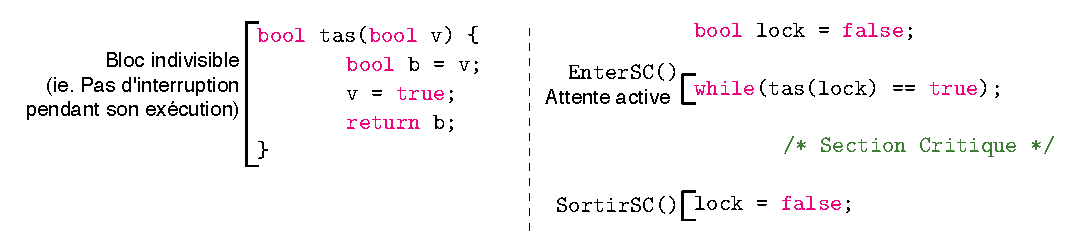
\includegraphics[scale=.85]{img/SC-tas} 
\end{figure}

\begin{figure}[h!]
	\center
	\vspace{-30pt}
	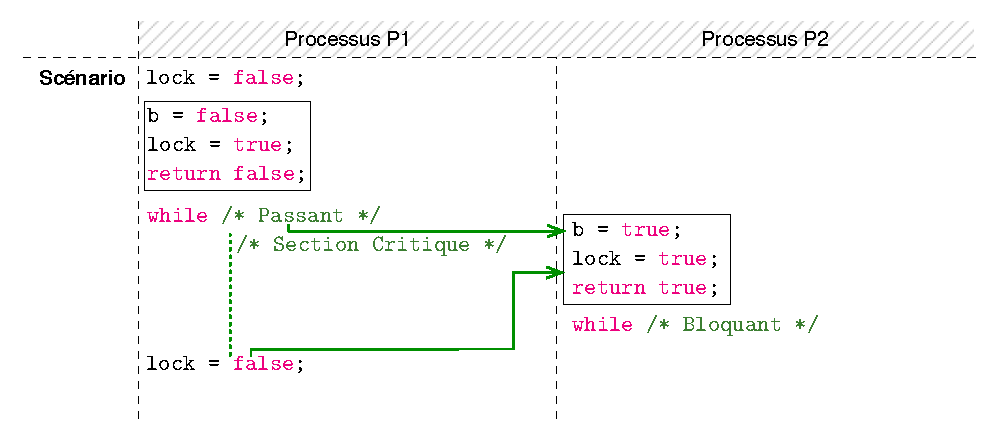
\includegraphics[scale=.85]{img/SC-tas-scenario}   
	\vspace{-30pt}
\end{figure}

\paragraph{Problèmes de performance} % (fold)

Problème de performance des solution à base d'attente active.
\begin{figure}[h!]
	\center
	\vspace{-10pt}
	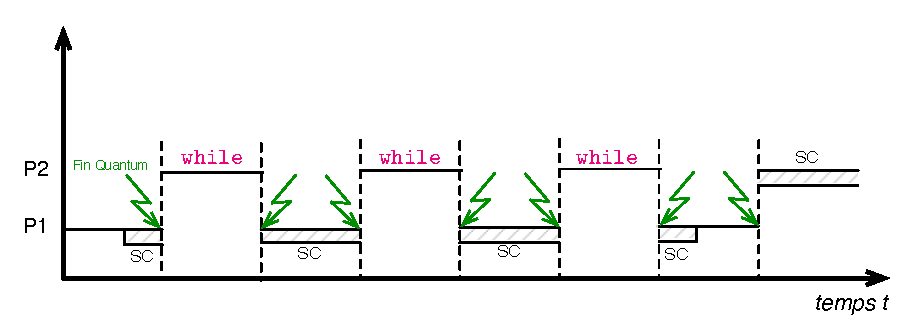
\includegraphics[scale=.85]{img/SC-perf}      
	\vspace{-30pt} 
\end{figure}

Ces solutions sont environ 2 fois plus lentes que les solutions sans attente active.

\section{Sémaphores}

Les sémaphores permettent d'éviter les attentes actives.
\subsection{Suspension/Réveil}

Considérons deux primitives :\begin{itemize}
	\item \lstinline!sleep()! : endormir un processus (passe de l'état prêt à l'état bloqué) ;
	\item \lstinline!wakeup()! : réveiller un processus.
\end{itemize}

\begin{ex*}
	Soit le code suivant (Ne marche pas !! ) :
\begin{lstlisting}[numbers=left,numberstyle=\footnotesize]
if(tas(lock) == true)
	sleep();
/* Section critique */
lock = false;
wakeup();
\end{lstlisting}
\end{ex*}

\begin{figure}[h!]
	\center
	\vspace{-10pt}
	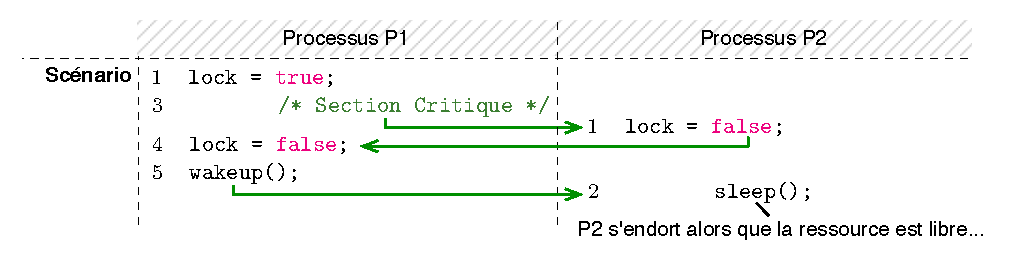
\includegraphics[scale=.85]{img/SC-sem}
\end{figure}

\subsection{Sémaphore : Dijkstra 76}

Un sémaphore est une structure gérée par le système d'exploitation permettant de contrôler l'accès à une ressource en évitant l'attente active. Celui-ci est composé de :
\begin{itemize}
	\item Un compteur (\lstinline!cpt!) = nombre de processus autorisés ;
	\item Une file d'attente (\lstinline!file!) pour les processus non autorisés.
\end{itemize}

Considérons les trois primitives indivisibles suivantes :

\begin{tabularx}{\linewidth}{lX}
	\lstinline!Init(sem, cpt)! & Création d'un sémaphore \lstinline!sem! dont le compteur est initialisé à \lstinline!cpt!.\\
	\lstinline!DS(sem)! & Destruction d'un sémaphore. Si la file n'est pas vide un traitement d'erreur doit être effectué.\\
	\lstinline!P(sem)! & Demande d'acquisition d'une ressource. Si aucune ressource n'est disponible, le processus est bloqué. Décrémente le compteur du sémaphore \lstinline!sem! $\Rightarrow$ demande un accès ``Puis-je ?'' (Bloquant) -- P : \emph{proboren} décrémenter NL\\
	\lstinline!V(sem)! & Libération d'une ressource. Si la file d'attente n'est pas vide, un processus est débloqué. Incrémente le compteur du sémaphore \lstinline!sem! $\Rightarrow$ libère un accès ``Vas-y !'' :  Reveil (non Bloquant) -- V : \emph{verhogen} incrémenter NL\\
\end{tabularx}

\begin{lstlisting}
Init (int val, SEM s){
	s.cpt = val;
	s.file = VIDE;
}
\end{lstlisting}
\begin{rem*}
	Attention \lstinline!val >= 0!
\end{rem*}

Les fonctions \lstinline!P! et \lstinline!V! sont des blocs indivisibles de code. Elles ne doivent pas être interrompues.
\begin{lstlisting}[multicols=2, tabsize=4]
P(SEM s){
	s.cpt --;
	if(s.cpt < 0){
		inserer(processus_courant, s.file);
		sleep();
	}
}

V(SEM s){
	s.cpt ++;
	if(s.cpt <= 0){
		p = retirer(s.file);
		wakeup(p);
	}
}
\end{lstlisting}

A propos de la valeur \lstinline!cpt! :\begin{itemize}
	\item \lstinline!cpt >= 0! : \lstinline!cpt! correspond au nombre de processus autorisés à accéder à la section critique ;
	\item \lstinline!cpt < 0! : \lstinline!|cpt|! est le nombre de processus bloqués dans la file.
\end{itemize}

\section{Problèmes de synchronisation classiques}
\subsection{Exclusion mutuelle}

\begin{def*}[Exclusion mutuelle]
	Autoriser un seul processus à la fois à accéder à la section critique.
\end{def*}

Soit un sémaphore \lstinline!MUTEX! initialisé de la façon suivante : \lstinline!init(MUTEX, 1);!

\begin{figure}[h!]
	\center
	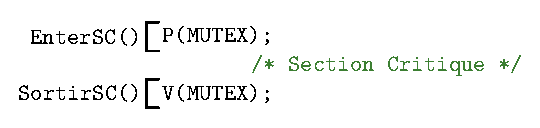
\includegraphics[scale=.85]{img/MUTEX}
\end{figure}

\subsection{Barrière de synchronisation}

\begin{def*}[Barrière de synchronisation]
	Un processus attend les autres à un point de synchronisation : la barrière.
\end{def*}

\begin{figure}[h!]
	\center
	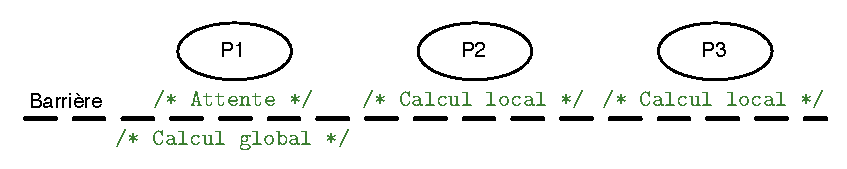
\includegraphics[scale=.85]{img/barriere1}
\end{figure}

Considérons deux sémaphores : \begin{itemize}
\item Un sémaphore S1 pour attendre le processus P2 ;
\item Un sémaphore S2 pour attendre le processus P3.
\end{itemize}

\begin{figure}[h!]
	\center
	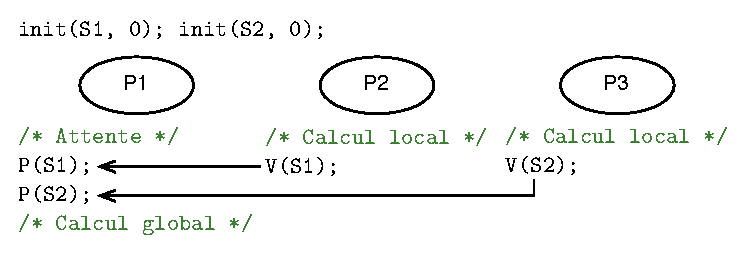
\includegraphics[scale=.85]{img/barriere2}
\end{figure}

\begin{figure}[h!]
	\center
	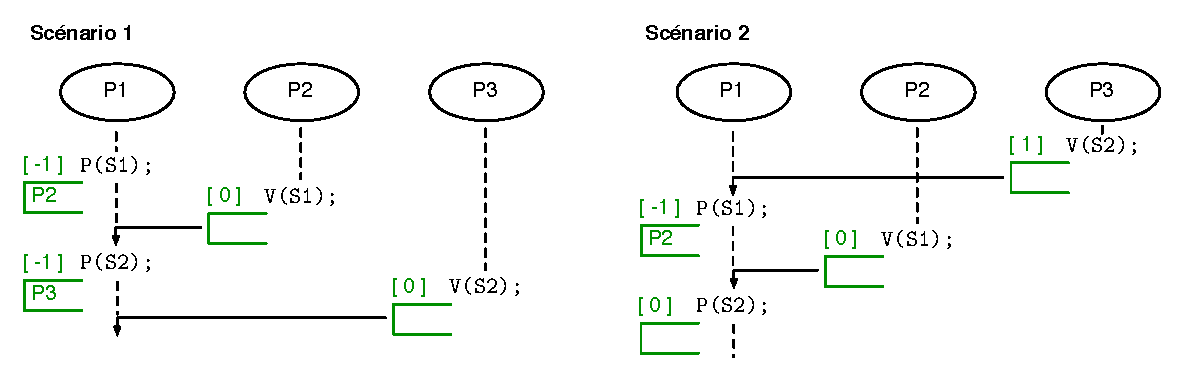
\includegraphics[scale=.85]{img/barriere3}
	\vspace{-10pt}
\end{figure}                                 

\begin{rem*}
	Il y a un compteur propre à chaque sémaphore. En général, il faut autant de \lstinline!P! que de \lstinline!V!.
\end{rem*}

\subsection{Producteur / consommateur}
Considérons un tampon $T$ partagé avec $N$ cases. Rôles des processus : \begin{itemize}
\item Processus producteurs : produisent dans $T$ ;
\item Processus consommateurs : consomment dans $T$.
\end{itemize}

\begin{figure}[h!]
	\center
	\vspace{-10pt}
	\includegraphics[scale=.85]{img/prod-cons}
	\vspace{-15pt}
\end{figure}

Gestion des indices \lstinline!ir! (commun aux consommateurs) et \lstinline!id! (commun aux producteurs) liés au tampon.
\begin{figure}[h!]
	\center
	\vspace{-20pt}
	\includegraphics[scale=.55]{img/multiprod-cons}
	\vspace{-10pt}
\end{figure}

Les producteurs sont bloqués si le tampon est plein $\Rightarrow$ un sémaphore \lstinline!Sprod! est alors nécessaire pour bloquer les producteurs : \lstinline!init(Sprod, 1);!

Les consommateurs sont bloqués si le tampon $T$ est vide $\Rightarrow$ un sémaphore \lstinline!Scons! est alors nécessaire pour bloquer les consommateurs : \lstinline!init(Scons, 0);!

\begin{figure}[h!]
	\center
	\vspace{-10pt}
	\includegraphics[scale=.85]{img/prod-cons2}
	\vspace{-10pt}
\end{figure}

Les variables \lstinline!id! et \lstinline!ir! sont partagées. De plus, nous souhaitons avoir une exécution la plus parallèle possible.

Considérons alors les sémaphores suivants :\begin{itemize}
	\item Les sémaphores \lstinline!MUTEXP! et \lstinline!MUTEXC! d'exclusion mutuelle pour respectivement les processus producteurs et les processus consommateurs, initialisés à 1 : \lstinline!init(MUTEXP, 1)! et \lstinline!init(MUTEXC, 1)! ;
	\item Le tableau de sémaphores \lstinline!C[1..n]! de taille \lstinline!n! et initialisés à 1 : \lstinline!for(i=0; i<n; i++)  init(C[i], 1);!. Avec ce tableau, un producteur en train de produire un message n'empêche pas d'autres producteurs d'acquérir des cases vides. De plus, il permet de garantir qu'un producteur ne produira pas dans une case en train d'être consommée.
\end{itemize}

Code des fonctions \lstinline!deposer()! et \lstinline!retirer()! satisfaisant aux conditions liées au problème.

\begin{lstlisting}[multicols=2,tabsize=4]
void deposer(message * m) {
	int i;
	P(MUTEXP);
		i = id; id = (id+1) % n;
		P(C[i]);
	V(MUTEXP);
	T[i] = m;
	V(C[i]);	
} 

message * retirer() {
	int i;
	P(MUTEXC);
		i = ir; ir = (ir+1) % n;
		P(C[i]);
	V(MUTEXC);
	message * m = T[i];
	V(C[i]);
	return m;
}
\end{lstlisting}
\vspace{-30pt}

\subsection{Lecteur / écrivain}
Un fichier est partagé par des processus lecteurs et écrivains.

Contraintes. $N$ lecteurs et 0 écrivain ou (XOR) un écrivain et 0 lecteur.

\begin{figure}[h!]
	\center
	\vspace{-10pt}
	\includegraphics[scale=.85]{img/lec-ecr}
	\vspace{-15pt}
\end{figure}

	Le premier lecteur verrouille le fichier en écriture et le dernier lecteur déverrouille le fichier en écriture $\Rightarrow$ Variable partagée comptant le nombre de lecteurs en train d'accéder au fichier : \lstinline!int nblect = 0;!

Sémaphores nécessaires : \begin{itemize}
	\item Un \lstinline!MUTEX! pour protéger la variable \lstinline!nblect! : \lstinline!init(MUTEX, 1);!
	\item Un sémaphore \lstinline!E! pour bloquer les écrivains (un écrivain à la fois peut accéder au fichier) : \lstinline!init(E, 1);! 
\end{itemize}

\begin{pb*}
	Il existe un risque de famine pour l'écrivain.
\end{pb*}
\vspace{-10pt}
\begin{lstlisting}[multicols=3,tabsize=4]
OuvreLecture() {
	P(MUTEX);
	nblect++;
	if(nblect == 1) P(E);
	V(MUTEX);
}

FermeLecture() {
	P(MUTEX);
	nblect--;
	if(nblect == 0) V(E);
	V(MUTEX);
}

OuvreEcriture() {
	P(E);
}
FermeEcriture() {
	V(E);
}	
\end{lstlisting}
\vspace{-10pt}


Utilisation d'une file (FIFO) pour assurer l'équité dans l'accès des processus à la section critique : lors de leur arrivée, tous les processus sont rangés dans une même file. Utilisation d'un sémaphore \lstinline!FILE! tel que \lstinline!init(FILE, 1)!. \begin{itemize}
	\item Extraction d'un écrivain ;
	\item Extraction du premier lecteur d'un groupe : autoriser les lecteurs suivant dans la file jusqu'à ce que le processus en tête de file soit un écrivain. 
\end{itemize}

\begin{lstlisting}[multicols=3,tabsize=4]
OuvreLecture() {
	P(FILE);
		P(MUTEX);
		nblect++;
		if(nblect == 1) P(E);
		V(MUTEX);
	V(FILE);
}

FermeLecture() {
	P(MUTEX);
	nblect--;
	if(nblect == 0) V(E);
	V(MUTEX);
}

OuvreEcriture() {
	P(FILE);
	P(E);
}
FermeEcriture() {
	V(E);
	V(FILE);
}	
\end{lstlisting}

\chapter{Gestion de la mémoire}
\section{Introduction}

Organisation de la mémoire.

\begin{figure}[h!]
	\center
	\vspace{-10pt}
	\includegraphics[scale=.85]{img/memoire-org}
\end{figure}

\section{Mémoire linéaire}

Avec la mémoire linéaire, les processus occupent des espaces contigus en mémoire. La totalité du programme et les données d'un processus doivent être chargées en mémoire pour pouvoir exécuter le processus. 

\subsection{Mono-programmation}
En mono-programmation, il n'y a qu'un seul processus en mémoire.
Un registre barrière est testé par le processeur (CPU) pour vérifier, à chaque accès mémoire, la validité des adresses soumises au processeur.

\begin{figure}[h!]
	\center
	\vspace{-10pt}
	\includegraphics[scale=.85]{img/mem-mono-prg}
\end{figure}

La partie du processeur qui gère la mémoire est la MMU (\emph{Memory Management Unit}).

\subsection{Multi-programmation}
En multi-programmation, plusieurs processus partagent la mémoire.
Les processus peuvent être relogeables (ie. Leur emplacement peut changer d'une exécution à une autre).

\begin{figure}[h!]
	\center
	\vspace{-10pt}
	\includegraphics[scale=.85]{img/mem-multi-prg}
\end{figure} 

De ce fait, les adresses sont relatives par rapport au début du processus. Il existe donc des mécanismes de traduction d'adresses relative en adresse physique (traduction effectuée par la MMU).
\begin{figure}[h!]
	\center
	\vspace{-10pt}
	\includegraphics[scale=.85]{img/MMU}
\end{figure}

Traduction relative $\Rightarrow$ physique par le CPU (MMU)
Positionnement registre de base fait par le système à la commutation de processus

\subsection{Allocation mémoire}
L'allocation mémoire est gérée par le système.
\begin{obj*}
 	Trouver un emplacement contigu en mémoire au moment de la création d'un processus.\\
	$\Rightarrow$ Le système maintient donc une liste des emplacements libres (\emph{freelist}).
\end{obj*} 

\begin{figure}[h!]
	\center
	\vspace{-20pt}
	\includegraphics[scale=.85]{img/mem-sys}
	\vspace{-10pt}
\end{figure}

Il existe trois stratégies d'allocation :
\begin{description}
	\item [\emph{First fit}] Choisir dans la liste le premier emplacement qui convient (taille > taille processus alloué).
	 
Avantages / inconvénients : \begin{itemize}
	\Pitem Simple ;
	\Citem Tendance à l'émiettement au début de la mémoire (miette : emplacement trop petit) ;
	\Citem Ne minimise pas le nombre de trous (emplacements).
	\begin{figure}[h!]
		\center
		\vspace{-10pt}
		\includegraphics[scale=.85]{img/firstfit}
		\vspace{-15pt}
	\end{figure}
\end{itemize}

	\item [\emph{Best fit}] Choisir l'emplacement qui convient le mieux (l'emplacement qui minimise le résidu).
	
	\begin{figure}[h!]
		\center
		\vspace{-10pt}
		\includegraphics[scale=.85]{img/bestfit}
		\vspace{-15pt}
	\end{figure}

Avantages / inconvénients :\begin{itemize}
	\Pitem Meilleure utilisation de la mémoire, moins de trous, \emph{freelist} plus petite) ;
	\Citem Plus complexe : parcourir toute la liste ;
	\Citem Tendance à un fort émiettement (si taille du résidu > 0).
\end{itemize}

	\item [\emph{Worst fit}] Choisir l'emplacement le plus grand $\Rightarrow$ Maximiser le résidu.
	
	\begin{figure}[h!]
		\center
		\vspace{-10pt}
		\includegraphics[scale=.85]{img/worstfit}
		\vspace{-15pt}
	\end{figure}
	
	Avantages / inconvénients :\begin{itemize}
		\Pitem Moins de miettes;
		\Citem Plus de trous dans la mémoire.
	\end{itemize}
\end{description}

Brenchmarks : les stratégies \emph{First fit} et \emph{Best fit} sont les meilleures (\emph{First fit} > \emph{Best fit} $>>$ \emph{Worst fit}).

\begin{def*}[Fragmentation interne]
	Si la taille d'un fichier n'est pas un multiple de la taille d'un bloc (ie. \lstinline&taille_fichier % taille_bloc != 0&), alors le système de fichiers allouera un nouveau bloc qui ne sera pas rempli entièrement, gaspillant ainsi de l'espace disque en provoquant de l'émiettement.
\end{def*}
\begin{def*}[Fragmentation externe]
	Fait d'avoir les blocs constituant le fichier répartis de façon non contiguë sur tout le disque, réduisant ainsi les performances d'accès à ce fichier, du fait de l'augmentation des mouvements des têtes de lecture du disque nécessaire à l'accès à ce fichier.
\end{def*}

\begin{pb}
	 Si trop d'émiettement (quelle que soit la stratégie utilisée), alors l'allocation n'est plus possible. Il faut alors réorganiser la mémoire avec un compactage / défragmentation :
	\begin{figure}[h!]
		\center
		\vspace{-15pt}
		\includegraphics[scale=.85]{img/defragmentation}
		\vspace{-20pt}
	\end{figure}
\end{pb}

\begin{pb}
	Le nombre de processus limité est directement proportionnel à la capacité de la mémoire physique.
\end{pb}
\begin{idee*}
	 Définir une zone de disque particulière comme extension de la mémoire (beaucoup plus lent : rapport de $100\,000$ à $1\,000\,000$)  $\Rightarrow$ zone de swap.
\end{idee*}
\begin{figure}[h!]
	\center
	\vspace{-10pt}
	\includegraphics[scale=.85]{img/swap}
	\vspace{-20pt}
\end{figure}

\subsection{Stratégie de \emph{swap}}

\begin{description}
	\item [\emph{Swap-out} (déchargement)] \hfill \begin{itemize}
		\item Intervient en cas de saturation mémoire ;
		\item Choisir un processus ``victime'' selon les critères suivants :
		\begin{itemize}
			\item Un processus à l'état \textbf{bloqué} ;
			\item Durée à l'état bloqué (un processus bloqué depuis longtemps);
			\item Taille (gros processus en priorité).
		\end{itemize}
	\end{itemize}
	\item[\emph{Swap-in} (chargement)] Dès qu'un processus ``swapé'' redevient prêt, il est rechargé en mémoire.\\
	Il y a éventuellement des déchargements de d'autres processus bloqués.
\end{description}

\section{Mémoire virtuelle}
\begin{idee*}
	Présence non contiguë et partielle des processus en mémoire. La traduction adresse virtuelle  $\Rightarrow$ adresse physique est effectuée par la MMU (\emph{Memory Management Unit}) qui se trouve au niveau du processeur.
\end{idee*}

\begin{figure}[h!]
	\center
	\vspace{-20pt}
	\includegraphics[scale=.7]{img/mem-virtuelle}
	\vspace{-30pt}
\end{figure}

\subsection{Mémoire segmentée}
Les processus sont découpés en \textbf{segments}. Un segment représente une zone mémoire pour la tâche. Il est associé à un aspect spécifique de la représentation de la tâche en mémoire (eg. code, données, pile, etc.). Un segment est chargé entièrement dans les zones de mémoire contiguës.

\begin{def*}[Segment]
Une suite d'emplacements \textbf{consécutifs} en mémoire et de \textbf{taille variable}.
\end{def*}

\begin{ex*}
	Il existe trois segments :
	\begin{itemize}
		\item Un segment code (\lstinline!.text!);
		\item Un segment pile (\lstinline!.stack!) ;
		\item Un segment données (\lstinline!.data!).
	\end{itemize}
\end{ex*}

La traduction nécessite une table des segments par \textbf{processus}.

\begin{figure}[h!]
	\center
	\vspace{-10pt}
	\includegraphics[scale=.85]{img/ts}
\end{figure}

Entrée de la table des segments se présente sous la forme : \lstinline!<P, Droits, Taille, Base>! :
\begin{itemize}
	\item \lstinline!P! : présence (0 : non présent, 1 : présent) ;
	\item \lstinline!droits! : R (\emph{Read}), W (\emph{Write}), X (\emph{eXecutable}).
\end{itemize}

\vspace{5pt}
La MMU (processeur) vérifie pour un couple \lstinline!<segment, offset>! :
\begin{itemize}
	\item \lstinline!Presence == 1 ?!  $\Rightarrow$ 0  $\Rightarrow$ IT défaut de segment (système) ;
	\item \lstinline!Droits OK ?!  $\Rightarrow$ Problème  $\Rightarrow$ violation segment (système) ;
	\item \lstinline!offset > taille!  $\Rightarrow$ Non $\Rightarrow$ IT débordement mémoire (système) ;
	\item Traduction (matériel).
\end{itemize}

Avantages / inconvénients de la mémoire segmentée : \begin{itemize}
	\Pitem Partage de segment en lecture.
	\begin{ex*}
	Les codes P1, P2 partagent \lstinline!gcc! :
	\begin{figure}[h!]
		\center
		\vspace{-10pt}
		\includegraphics[scale=.6]{img/partage-gcc}
	\end{figure}
	\end{ex*}
	\Citem Allocation des segments : trouver un emplacement consécutif en mémoire physique (\emph{First fit}, \emph{Best fit}, \emph{Worst fit}).\\
 $\Rightarrow$ Problème de fragmentation + compactage.
\end{itemize}

\subsection{Mémoire paginée}
Mémoire virtuelle (espace virtuel) découpée en \textbf{pages} de \textbf{tailles fixes}.

Mémoire physique découpée en cases (\emph{frames})
Taille page = taille case.
\begin{figure}[h!]
	\center
	\vspace{-10pt}
	\includegraphics[scale=.6]{img/virt-phy}
\end{figure}

La traduction adresse virtuelle  $\Rightarrow$ adresse physique est effectuée par la MMU.
\begin{figure}[h!]
	\center
	\vspace{-10pt}
	\includegraphics[scale=.6]{img/trad-phy-virt}
\end{figure}
 
\begin{rem*}
	La taille de page doit être une puissance de 2.\\
	L'adresse physique est égale à \lstinline!case * taille!.
\end{rem*}

\begin{ex*}
Soit une taille de page égale à 512 octets et une adresse virtuelle de base égale à $2\,050$ :
\begin{itemize}
	\item \lstinline!page! = $2\,050 \div 512 = 4$ ;
	\item \lstinline!offset! = $2\,050 \bmod 512 = 2$.
\end{itemize}
\end{ex*}

Entrée de la table des pages : 
\lstinline!<Presence, droits, evincee, modifiee, Case>!
\begin{itemize}
	\item \lstinline!Present! : 0 : non présent, 1 : présent ;
	\item \lstinline!droits! : RWX;
	\item \lstinline!evincer! : 0 : non verrouillée, 1 : verrouillée ;
	\item \lstinline!modifiee! : 0 : non modifiée, 1 : modifiée.
\end{itemize}
Une version abrégée : \lstinline!<P, droits, V, M, Case>!

\begin{rem*}
    Les champs sont dépendant de l'architecture du processeur. 
\end{rem*}

Les pages sont chargées \textbf{à la demande} au fur et à mesure des accès.
\begin{figure}[h!]
	\center
	\vspace{-10pt}
	\includegraphics[scale=.5]{img/pages-load}
\end{figure}
Accès à une page avec \lstinline!P = 0! $\Rightarrow$ MMU lève l'interruption ``défaut de page'' (\emph{page fault}).

Le système maintient une liste de cases libres.\\
 $\Rightarrow$ Lorsque le nombre de cases libre est trop faible, le système doit libérer des cases en déchargeant une partie des cases ramenées en mémoire sur disque, dans la zone de swap.

\subsection{Remplacement des pages}
Permet de réguler l'activité mémoire. Ce mécanisme intervient en cas de pénurie de mémoire.

\begin{obj*}
	Il y a deux objectifs à atteindre :\begin{itemize}
		\item Choisir une page (victime) à évincer sur le disque, dans la zone de swap (si la page a été modifiée) ;
		\item Utiliser la case libérée.
	\end{itemize} 
\end{obj*}

\subsubsection{Algorithmes de remplacement de page}
\begin{obj*}
	Choisir une bonne victime en minimisant le nombre de défauts de page.
\end{obj*} 

Il existe trois types d'algorithme.
\begin{description}
	\item [Optimal] (théorique) : choisir la page qui sera utilisée le plus tardivement.
	$\Rightarrow$ Connaissance du futur.
	\item [FIFO] Choisir la page la plus vieille.
	\begin{itemize}
		\Pitem Simple à implémenter :
		\begin{figure}[h!]
			\center
			\vspace{-10pt}
			\includegraphics[scale=.5]{img/pages-FIFO}
		\end{figure}
		\Citem Peu performant car on ne prend pas en compte l'utilisation des pages.
	\end{itemize}
	\item [LRU (\emph{Least Recently Used})] Choisir la page la moins récemment utilisée.
	\begin{idee*}
	Utiliser la propriété de \textbf{localité temporelle} : une page utilisée il y a longtemps a peu de chance d'être utilisée dans un futur proche.

	$\Rightarrow$ Notion de \emph{working set} : ensemble des pages les plus utilisées.
	\end{idee*}
	\begin{itemize}
	\Pitem Bon choix (défauts de pages faibles) ;
	\Citem Très (trop) coûteux à implémenter : nécessité de tracer tous les accès en mémoire.
\end{itemize}
\begin{figure}[h!]
	\center
	\vspace{-10pt}
	\includegraphics[scale=.5]{img/pages-LRU}
\end{figure} 
\end{description}

Il existe une approximation LRU en NRU (\emph{Not Recently Used})\\
$\Rightarrow$ Ajout de bits supplémentaires dans la table des pages :\begin{itemize}
	\item \emph{Reference bit} (\lstinline!R!) positionné à 1 par la MMU à chaque accès de page (en lecture ou en écriture) ;
	\item \emph{Acces bit} (\lstinline!A!) positionné à 1 par la MMU à chaque modification de la page concernée (écriture).
\end{itemize}

%maybe in an evironment...
\begin{ppe*}[NRU -- \emph{Not Recently Used}]
	\hfill
	\begin{itemize}
		\item Le système re-positionne régulièrement les bits \lstinline!R! à 0 ;
		\item \lstinline!R! testés plus tard, si \lstinline!R! toujours à 0 $\Rightarrow$ page plus récemment utilisée.
	\end{itemize}

	\begin{ex*}
	Clock (UNIX)
	\begin{figure}[h!]
		\center
		\vspace{-10pt}
		\includegraphics[scale=.85]{img/UNIX-clock}
	\end{figure}
	\end{ex*}	
\end{ppe*}

Deux types de mémoire pour l'instant :\begin{itemize}
	\item \textbf{Mémoire paginée} : espace d'adressage du processus découpé en blocs (pages) de taille fixe.
	\item \textbf{Mémoire segmentée} : espace d'adressage du processus découpé en blocs (segments) de tailles variables.
\end{itemize}

\section{Mémoire segmentée paginée}
\begin{idee*}
	 Lever la contrainte de contiguïté des segments en mémoire physique. $\Rightarrow$ Segments découpés en pages.
\end{idee*}

Schéma ``classique'' : une table des pages par segment : \begin{itemize}
	\item Adresse virtuelle définie par : \lstinline!<segment, offset>! ;
	\item Déplacement à l'intérieur du segment défini par : \lstinline!<page, offset>!.
\end{itemize}

\begin{figure}[h!]
	\center
	\vspace{-10pt}
	\includegraphics[scale=.6]{img/segmente-pagine}
	\vspace{-20pt} 
\end{figure}

\paragraph{Cache des adresses traduites : TLB (\emph{Translation Look-Aside Buffer})}

Mémoire associative interne au processeur (pas en RAM) pour mémoriser les pages déjà traduites.

\begin{figure}[h!]
	\center
	\vspace{-10pt}
	\includegraphics[scale=.85]{img/TLB}
\end{figure}

\begin{itemize}
	\item TLB consultée à chaque traduction ;
	\item Mise à jour de la TLB : \begin{itemize}
		\item Nouvelle page ;
		\item Vidage (flush) des caches à chaque commutation de processus (pas le cas des threads).
		\begin{figure}[h!]
			\center
			\vspace{-10pt}
			\includegraphics[scale=.85]{img/commutation-tlb}
		\end{figure}
	\end{itemize}
\end{itemize}

\begin{ex*}
	Dans le processeur Intel 32 bits, la mémoire est \textbf{segmenté paginée} : une table des segments par processus : LDT (\emph{Local Descriptor Table}).
	
	\begin{figure}[h!]
		\center
		\vspace{-15pt}
		\includegraphics[scale=.85]{img/traduction-etapes}
		\vspace{-15pt}
	\end{figure}
		 
	Les pages ont une taille de 4 Ko, donc l'\emph{offset} est codé sur 12 bits. Puisque l'adresse est codée sur 32 bits, le numéro de page est codé sur 20 bits, ce qui donne lieu à $2^{20}$ pages, soit plus de 1 million de pages potentielles.\\
	Une table des pages à 1 million d'entrées aurait une taille égale à $2^{20}\times 4 = 2^{22}$ octets = 4 Mo.
	
	Les architectures Intel utilise donc des pages multi-niveaux (2 pour l'architecture 32 bits, jusqu'à 4 niveaux de pages pour les architectures à 64 bits).
	
	\begin{figure}[h!]
		\center
		\vspace{-15pt}
		\includegraphics[scale=.85]{img/pagination-2-niv}
		\vspace{-20pt}
	\end{figure}
   
\end{ex*}

\chapter{Entrées / sorties Disque}
\section{Définitions}

Il existe deux types de périphériques : 
\begin{description}
	\item [Mode bloc (disque)] Lecture / Ecriture par bloc de manière indépendante $\Rightarrow$ Mode adressable.
	\item [Mode caractère (console, imprimante, réseau)] Pas de structuration du flux $\Rightarrow$ Accès séquentiel.
\end{description}

Architecture d'un disque 
\begin{figure}[h!]
	\center
	\vspace{-10pt}
	\includegraphics[scale=.85]{img/HD}
\end{figure}

Accès aux données (piste, secteur) :
\begin{itemize}
	\item Positionnement sur la piste (\emph{seek time}) ;
	\item Attendre le passage du secteur sous la piste ;
	\item Transfert.
\end{itemize}

\section{Ordonnancement des requêtes d'E/S}
A chaque disque, est associée une file d'attente des requêtes (numéro de piste). Ces files d'attente sont gérées par le système à l'aide des pilotes/drivers.

\begin{obj*}
	Limiter les déplacements des têtes de lecture des disques durs.
\end{obj*}

\subsection{Premier arrivé, premier servi -- FIFO / FCFS}
Les requêtes sont servies dans l'ordre.

\begin{ex*}
	Supposons la tête de lecture sur la piste 53.\\ 
	Contenu de la file d'attente : 98, 183, 37, 122, 14, 124, 65, 67.
\end{ex*}

\begin{figure}[h!]
	\center
	\vspace{-10pt}
	\includegraphics[scale=.85]{img/hd-FIFO}
\end{figure}

\subsection{Plus court déplacement d'abord -- SSTF \emph{Shortest Seek Time First}}

\begin{figure}[h!]
	\center
	\vspace{-10pt}
	\includegraphics[scale=.85]{img/hd-SSTF}
\end{figure}

Avantages / inconvénients :
\begin{itemize}
	\Pitem Performant ;
	\Citem Risque de famine des requêtes lointaines.
\end{itemize}

\subsection{Algorithme à balayage (idem ascenseurs -- Look)}

Balayage du disque entre les deux requêtes les plus éloignées. Requêtes servies au passage de la tête de lecture. Il existe une variante : C-Look (\emph{Circular Look}).

\begin{figure}[h!]
	\center
	\vspace{-10pt}
	\includegraphics[scale=.85]{img/C-Look}
\end{figure}


\chapter{Systèmes de gestion de fichiers}

Un système de gestion de fichiers (FS -- \emph{file system}) est une façon de stocker les informations et de les organiser dans des fichiers sur ce que l'on appelle des mémoires secondaires (disque dur, CD-ROM, clé USB, SSD, disquette, etc.).

\section{Introduction}
\begin{figure}[h!]
	\center
	\vspace{-15pt}
	\includegraphics[scale=.85]{img/SGF}
	\vspace{-5pt}
\end{figure}

Un Système de Gestion de Fichiers doit pouvoir assumer plusieurs rôles :
\begin{itemize}
	\item Accès aux données : conversion \lstinline!<nom, offset>! en bloc sur disque ;
	\item Gestion de l'espace libre.
	\item Allocation de la place sur mémoires secondaires : les fichiers étant de taille différente et cette taille pouvant être dynamique, le SGF alloue à chaque fichier un nombre variable de granules de mémoire secondaire de taille fixe (blocs) ;
	\item Manipulation des fichiers : des opérations sont définies pour permettre la manipulation des fichiers par les programmes d’application, à savoir : créer/détruire des fichiers, insérer, supprimer et modifier un article dans un fichier ;
	\item Sécurité et contrôle des fichiers : le SGF permet le partage des fichiers par différents programmes d’applications tout en assurant la sécurité et la confidentialité des données. 
\end{itemize}

Un disque est divisé en partitions. Chaque partition du disque possède ses propres structures.\\
Une partition contient des fichiers regroupés en répertoires $\Rightarrow$ Ces fichiers et répertoires forment une arborescence.

\begin{figure}[h!]
	\center
	\vspace{-15pt}
	\includegraphics[scale=.7]{img/arborescenceSGF}
	\vspace{-15pt}
\end{figure}

Mode d'accès aux fichiers : 
\begin{description}
\item [Accès séquentiel] \hfill
\begin{itemize}
	\item Lecture d'un flux de données
	\item Ecriture en fin de fichier
\end{itemize}
\item [Accès indexé (direct)] Accès direct aux blocs
\end{description}

\begin{figure}[h!]
	\center
	\vspace{-15pt}
	\includegraphics[scale=.85]{img/acces-fichier}
	\vspace{-15pt}
\end{figure}

\section{Politique d'allocation}

On veut gérer l'allocation de données sur le disque pour les fichiers utilisateurs. Le disque est structuré en \textbf{blocs}. La politique d'allocation des blocs permet de définir la structuration des blocs de données du système de gestion de fichiers.

\subsection{Allocation contiguë (séquentielle)}
Un fichier est un ensemble de blocs sur le disque (pas forcément consécutifs). Si l'on veut optimiser d'accès séquentiel aux fichiers, il faut minimiser les déplacements de la tête de lecture du disque. De ce fait, il faut utiliser un bitmap pour gérer l'espace libre sur le disque afin d'avoir des fichiers alloués sur des blocs contigües.

\begin{figure}[h!]
	\center
	\vspace{-10pt}
	\includegraphics[scale=.75]{img/allocation-contigue}
	\vspace{-10pt}
\end{figure}

Avantages /inconvénients :
\begin{itemize}
	\Pitem Simple, performant (déplacement des têtes de lecture du disque dur) ;
	\Pitem Accès séquentiel direct : facilement implémentable ;
	\Citem Allocation : défragmentation régulière ;
	\Citem Changement de taille lourd.
\end{itemize}

\subsection{Allocation chainée}
Un fichier est considéré comme étant une suite de blocs chainés entre eux.

\begin{figure}[h!]
	\center
	\vspace{-15pt}
	\includegraphics[scale=.75]{img/allocation-chainee}
	\vspace{-20pt}
\end{figure}

Avantages/inconvénients :
\begin{itemize}
	\Pitem Allocation simple ;
	\Pitem Changement de taille ;
	\Pitem Accès séquentiel ;
	\Citem Pas d'accès direct ;
	\Citem Fiabilité : parte d'un bloc $\Rightarrow$ Perte de la fin du fichier.
	\begin{figure}[h!]
		\center
		\vspace{-15pt}
		\includegraphics[scale=.75]{img/allocation-chainee-inconvenient}
		\vspace{-15pt}
	\end{figure}
\end{itemize}

Il existe une variante à l'allocation chaînée : table d'allocation de fichiers ou FAT (\emph{File Allocation Table}).

\subsection{FAT (File Allocation Table}

La FAT (\emph{File Allocation Table}) est une structure de données permettant de gérer à la fois l'espace libre et l'espace alloué. Il s'agit d'un tableau avec une entrée par bloc stocké en début de partition.

Dans un répertoire, on trouve pour chaque fichier le numéro du premier bloc occupé par le fichier. L'entrée correspondante de la FAT contient l'adresse du 2\up{ème} bloc occupé, etc.\\
L'entrée de la FAT correspondant du dernier bloc occupé contient une valeur spéciale ``fin de fichier'' (EOF -- \emph{End Of File}). Les entrées correspondant aux blocs vides sont égales à 0.

En résumé, une entrée par bloc prend pour valeur :
\begin{itemize}
	\item 0 : bloc libre ;
	\item -1 : dernier bloc ;
	\item > 0 : numéro de bloc suivant (chainage).
\end{itemize}

\begin{figure}[h!]
	\center
	\vspace{-15pt}
	\includegraphics[scale=.85]{img/FAT}
	\vspace{-15pt}
\end{figure}

Avantages / inconvénients :
\begin{itemize}
	\Pitem Accès direct possible (lecture d'entrées de la FAT) ;
	\Pitem Fiabilité : réplication de la FAT ;
	\Citem Accès direct peu performant ;
	\Citem Déplacement de la tête de lecture : accès à la FAT en début de partition.
\end{itemize}

\subsection{Allocation indexée}
L'allocation indexée consiste à un index par fichier contenant la liste des blocs composant le fichier.

\subsubsection{Index simple}
Un bloc d'index est alloué par fichier.

\begin{figure}[h!]
	\center
	\vspace{-20pt}
	\includegraphics[scale=.85]{img/allocation-indexee}
	\vspace{-20pt}
\end{figure}

Avantages / inconvénients :
\begin{itemize}
	\Pitem Accès séquentiel/direct ;
	\Citem Perte d'un bloc par fichier $\Rightarrow$ Important car beaucoup de petits fichiers ;
	\Citem Taille limitée à la capacité du bloc d'index. 
\end{itemize}

\subsubsection{Index multi-niveau (UNIX)}

Dans le système de gestion des fichiers d'UNIX, à chaque fichier est associée une structure de données appelée \emph{inode}. Dans cette structure, on trouve une liste de blocs contenant 13 entrées :\begin{itemize}
	\item Les 10 premières entrées référencent des blocs de données sur le disque (\textbf{accès direct}) ;
	\item La 11\up{e} référence un bloc de contrôle sui référence des blocs de données (\textbf{simple indirection}) ;
	\item La 12\up{e} référence un bloc de contrôle qui référence des blocs de contrôle qui référencent des blocs de données (\textbf{double indirection}) ;
	\item La 13\up{e} référence un bloc de contrôle qui référence des blocs de contrôle qui référencent des blocs de contrôle qui référencent des blocs de données (\textbf{triple indirection}).
\end{itemize}

Chaque bloc de contrôle permet de référencer au maximum \textbf{128} blocs (de contrôle ou de données).\\
La taille max d'un fichier est alors donnée par la formule :
\[
	\left(10+128+128^2+128^3\right)\times 512 = 1082201088 \textrm{ octets} \geqslant 1\textrm{ Go}
\]

\begin{rem*}
	La taille d'un bloc de contrôle est de $128\times 4 = 512$ octets qui était la taille UNIX initiale d'un bloc.
\end{rem*}

Attributs d'un fichier selon la norme POSIX (métadonnées) :
\begin{itemize}
	\item La taille du fichier en octets ;
	\item Identifiant du périphérique contenant le fichier ;
	\item L'identifiant du propriétaire du fichier (UID) ;
	\item L'identifiant du groupe auquel appartient le fichier (GID) ;
	\item Le numéro d'\emph{inode} qui identifie le fichier dans le système de fichier ;
	\item Le mode du fichier (RWX) ;
	\item Timestamp pour :\begin{itemize}
		\item La date de dernière modification \lstinline!ctime! de l'inode (affichée par la commande \lstinline!stat! ou par \lstinline!ls -lc!, modification des droits du fichier) ;
		\item La date de dernière modification du fichier \lstinline!mtime! (affichée par le classique \lstinline!ls -l!) ;
		\item La date de dernier accès \lstinline!atime! (affichée par la commande \lstinline!stat! ou par \lstinline!ls -lu!).
	\end{itemize}
	\item Un compteur indiquant le nombre de liens physiques sur cet inode (\lstinline!Nlinks!) ;
	\item Liste des blocs compost le fichier.
\end{itemize}
Ces métadonnées forment une structure \emph{inode}.

\begin{rem*}
	Les inodes ne contiennent pas les noms de fichier.
\end{rem*}

\begin{figure}[h!]
	\center
	\vspace{-15pt}
	\hspace{-40pt}\centerline{\includegraphics[scale=.7]{img/inode}}
	\vspace{-15pt}
\end{figure}

Avantages / inconvénients:
\begin{itemize}
	\Pitem Accès rapide aux petits fichiers ;
	\Pitem Gestion des gros fichiers (simple, double, triple indirection) ;
	\Citem Accès aux blocs non uniforme.
\end{itemize}

\section{Gestion d'espace libre}

\begin{obj*}
	La gestion de l'espace libre (ie. des blocs qui sont libres) permet de trouver ces blocs libres.
\end{obj*}

\subsection{Liste chainée}
Une \emph{freelist} des blocs libres.

\begin{figure}[h!]
	\center
	\vspace{-15pt}
	\includegraphics[scale=.85]{img/freelist-blocs}
	\vspace{-15pt}
\end{figure}

Avantages / inconvénients :
\begin{itemize}
	\Pitem Simple à implémenter ;
	\Citem Fragile ;
	\Citem Peu performant pour des demandes groupées.
\end{itemize}

\subsection{Regroupement}
Un bloc spécial (\emph{superbloc}) contient (entre autres) :\begin{itemize}
	\item En première position (indice 0) : le numéro du prochain bloc contenant une liste de blocs libres ;
	\item De l'indice 1 à l'indice $N+1$ : une liste de $N$ blocs libres
\end{itemize}
De ce fait, chaque bloc contient les numéros de $N$ blocs libres.
\begin{figure}[h!]
	\center
	\vspace{-25pt}
	\includegraphics[scale=.85]{img/regroupement}
	\vspace{-50pt}
\end{figure}

Avantages / inconvénients :
\begin{itemize}
	\Pitem Fournir rapidement beaucoup de blocs libres ;
	\Pitem Faible occupation mémoire ;
	\Citem Difficile de fournir des blocs libres proches sur le disque $\Rightarrow$ Fragmentation importante.
\end{itemize}

\subsection{Vecteur linéaire (bitmap)}
Une entrée par bloc codée sur 1 bit :
\begin{itemize}
	\item 0 : bloc libre ;
	\item 1 : bloc occupé.
\end{itemize}

\begin{figure}[h!]
	\center
	\vspace{-15pt}
	\includegraphics[scale=.85]{img/bitmap}
	\vspace{-15pt}
\end{figure}

Allocation de $N$ blocs pour un même fichier : trouver une séquence de $N$ zéros dans le bitmap. Il existe plusieurs stratégies possibles : \emph{Best Fit}, \emph{First Fit}, \emph{Worst Fit}\dots

Avantages / inconvénients :
\begin{itemize}
	\Pitem Limite la fragmentation : il est possible d'allouer facilement $n$ blocs contigües (il suffit de maximiser le nombre de 0 consécutifs) ;
	\Citem Taille : importante pour les grosses partitions.
\end{itemize}

\end{document}